\begin{figure}
    \centering
    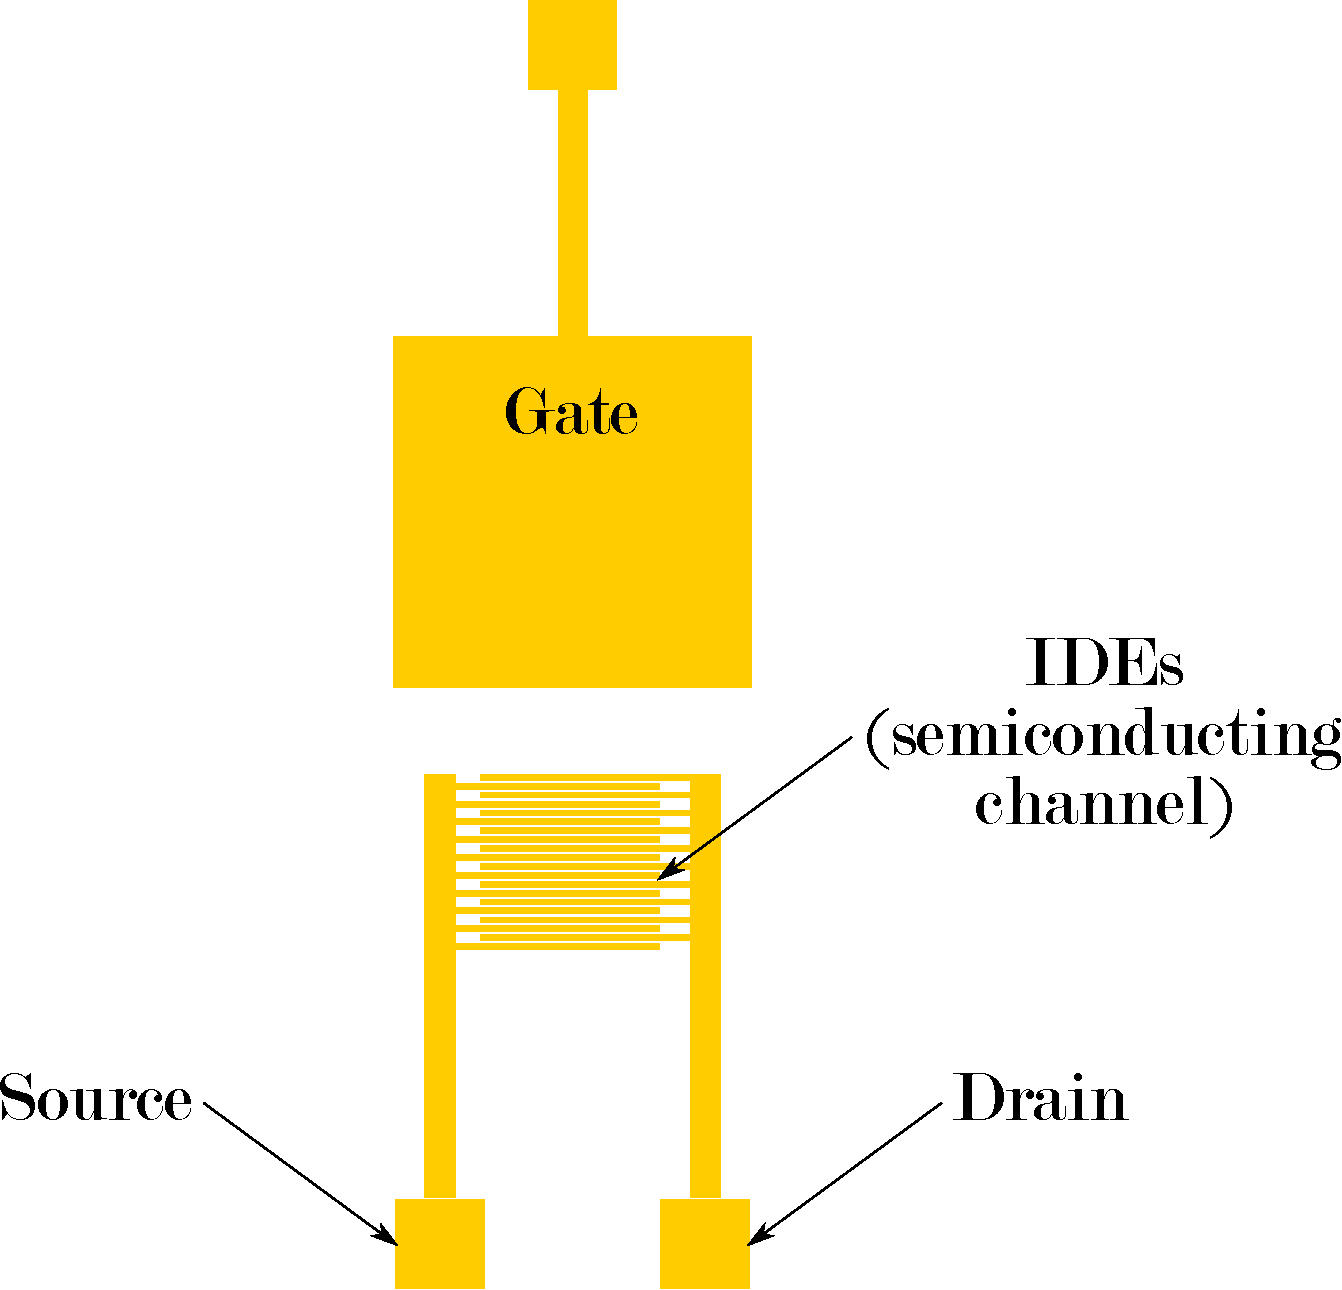
\includegraphics[width=0.3\textwidth]{figures/chapter3/EGFET/standardEGFET_scheme.pdf}
    \quad
    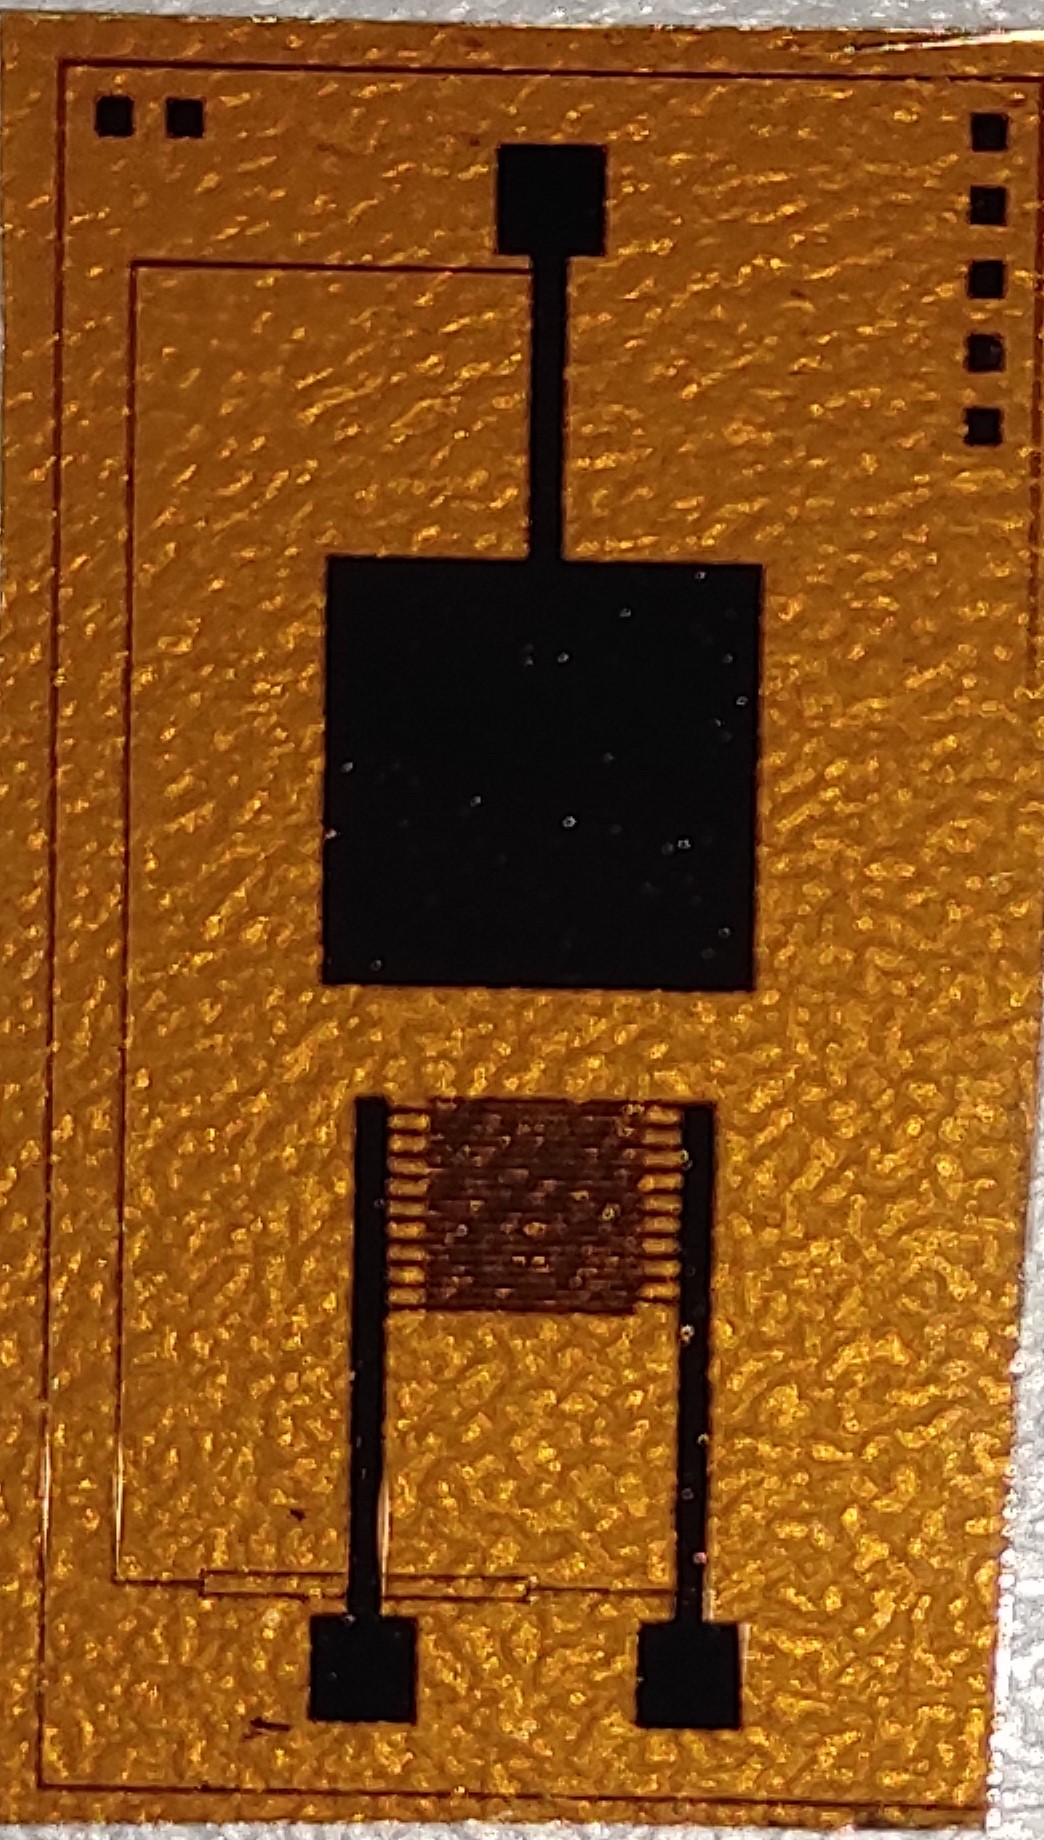
\includegraphics[width=0.16\textwidth]{figures/chapter3/EGFET/standardEGFET.jpg}
    \caption{The geometry of the standard EG-FET has been previously optimized by \citet{joshiUnderstanding2018}. The square gate has a side length of \SI{5.7}{\mm}, while the IDEs have a length of \SI{3}{\mm} and a height of \SI{100}{\um}. The channel length is \SI{50}{\um}, and due to the interdigitated design, the channel width amounts to \SI{57}{\mm}. The distance between the channel and gate is set to \SI{1.5}{\mm}.}
    \label{fig:standardEGFET}
\end{figure}

The standard EG-CNTFET geometry in Figure \ref{fig:standardEGFET} was based on the studies of \citet{joshiUnderstanding2018}, who evaluated different ratios between the gate area and the channel area; it was found that best performance was achieved by the configuration where the gate area was four times larger than the channel area. The IDEs are \SI{3}{\mm} long and \SI{100}{\um} high, with a channel width that amounts to \SI{57}{\mm}; this configuration results in a large $\frac{W}{L}$ ratio, which is linked to a high transconductance through Equation \eqref{eq:transconductance}. A big transconductance leads to an increased sensitivity of the device to small variations in gate potential, thus making it more responsive to changes in the applied voltage. Finally, a planar \SI{5.7}{\mm} $\times$ \SI{5.7}{\mm} gate electrode was employed.

The deposition of SWCNTs onto the devices was carried out following the protocol previously optimized by \citet{shkodraOptimization2023}, as described in Section \ref{sec:cntDeposition}. Following this protocol, 60 layers of SWCNTs were deposited, leading to a post-deposition \rds{} between \SIrange{1}{10}{\kohm}; in fact, it was observed by \citet{petrelliMethod2023} that this range is where the performance of this type of device is optimal. In addition, this step provided an initial skimming of the manufactured devices, in order to reduce device-to-device variability that could be detrimental to subsequent steps.

The devices that passed this screening were subjected to electrical characterization, by collecting transfer characteristics, according to the protocol given in Section \ref{sec:characterization}.

The first step was to determine the behavior of the as-manufactured devices, with the bare channel. This would provide a baseline against which modified devices could be compared in the hope of achieving better performance. To this end, the raw transfer curves were observed, without any processing (Figure \ref{fig:transferNoMem}), after which the variation of the ON current (\ion{}) was evaluated as a function of time (Figure \ref{fig:NormNoMem}). Normalization was performed by taking the \ion{} value at \vgs{}=\SI{-0.8}{\V} for each cycle and dividing it by the \ion{} of the first recorded transfer curve during that measurement sequence. This approach is useful to standardize the current variations across different devices, allowing a fair comparison of their performance. While the measured current was always considered, normalization helped in further mitigating the influence of device-to-device variation, thus facilitating the comparison among different devices, without interference from fabrication inconsistencies.
The observation of transfer characteristics shows that the \ids{} decreases progressively after each measurement cycle, although this trend is more clearly seen in the normalized \ion{} over time. This decrease indicates that there is a level of degradation of CNTs and that something occurs during their use that alters their functionality. This effect is not particularly relevant during the 60-minute measurement, though it can become a problem for longer measurements, as in the case of EG-CNTFET used as a transducer for a sensor. Calibration measurements, in fact, can take several hours; during this time there is a risk that the measured current will continuously decrease until it reaches \SI{0}{\uA}, making the measurements unreliable.

\begin{figure}
    \centering
    \subfloat[Transfer characteristics]{%
        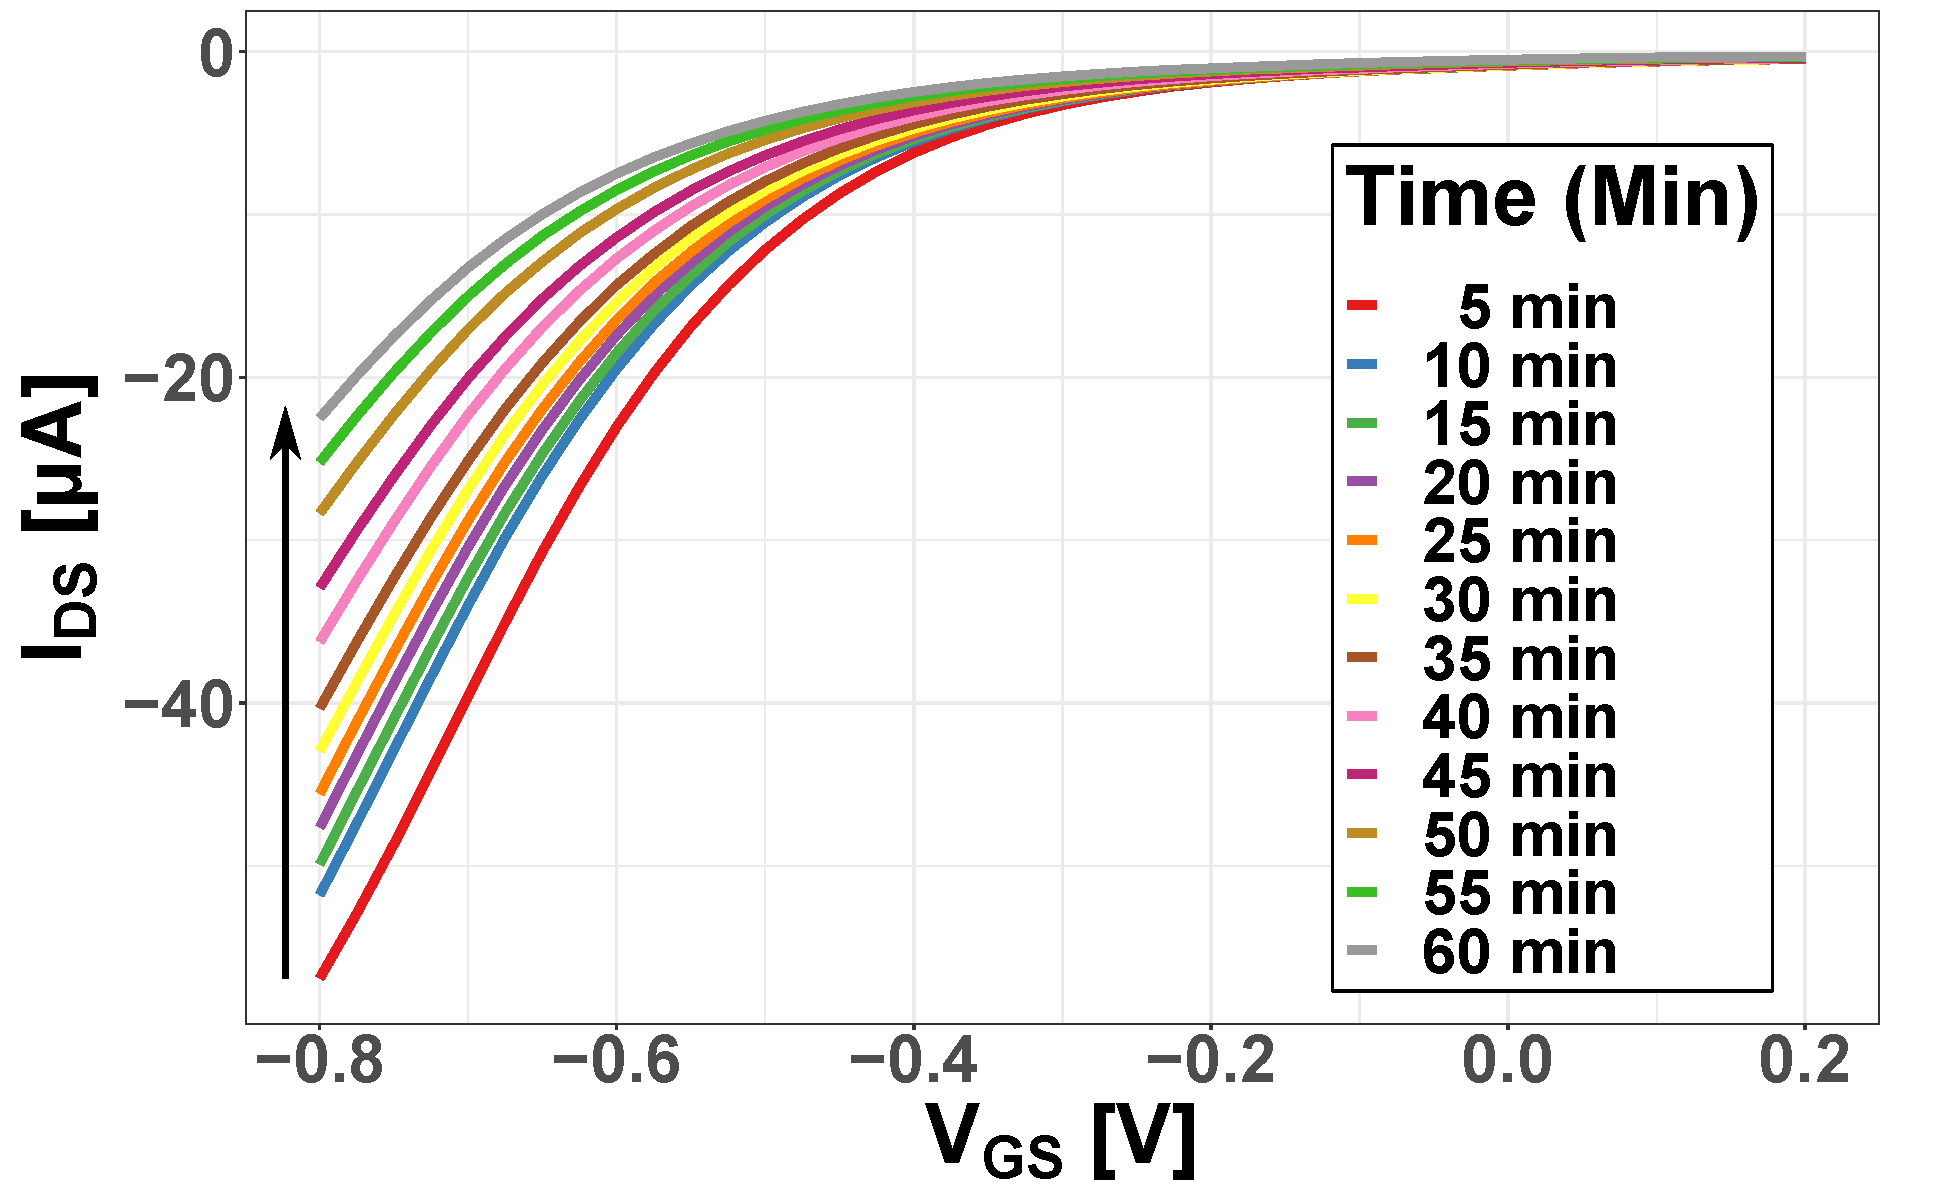
\includegraphics[width=0.45\textwidth]{figures/chapter3/EGFET/transferNoMem.pdf}%
        \label{fig:transferNoMem}
    }
    \quad
    \subfloat[Normalized \ion{}]{%
        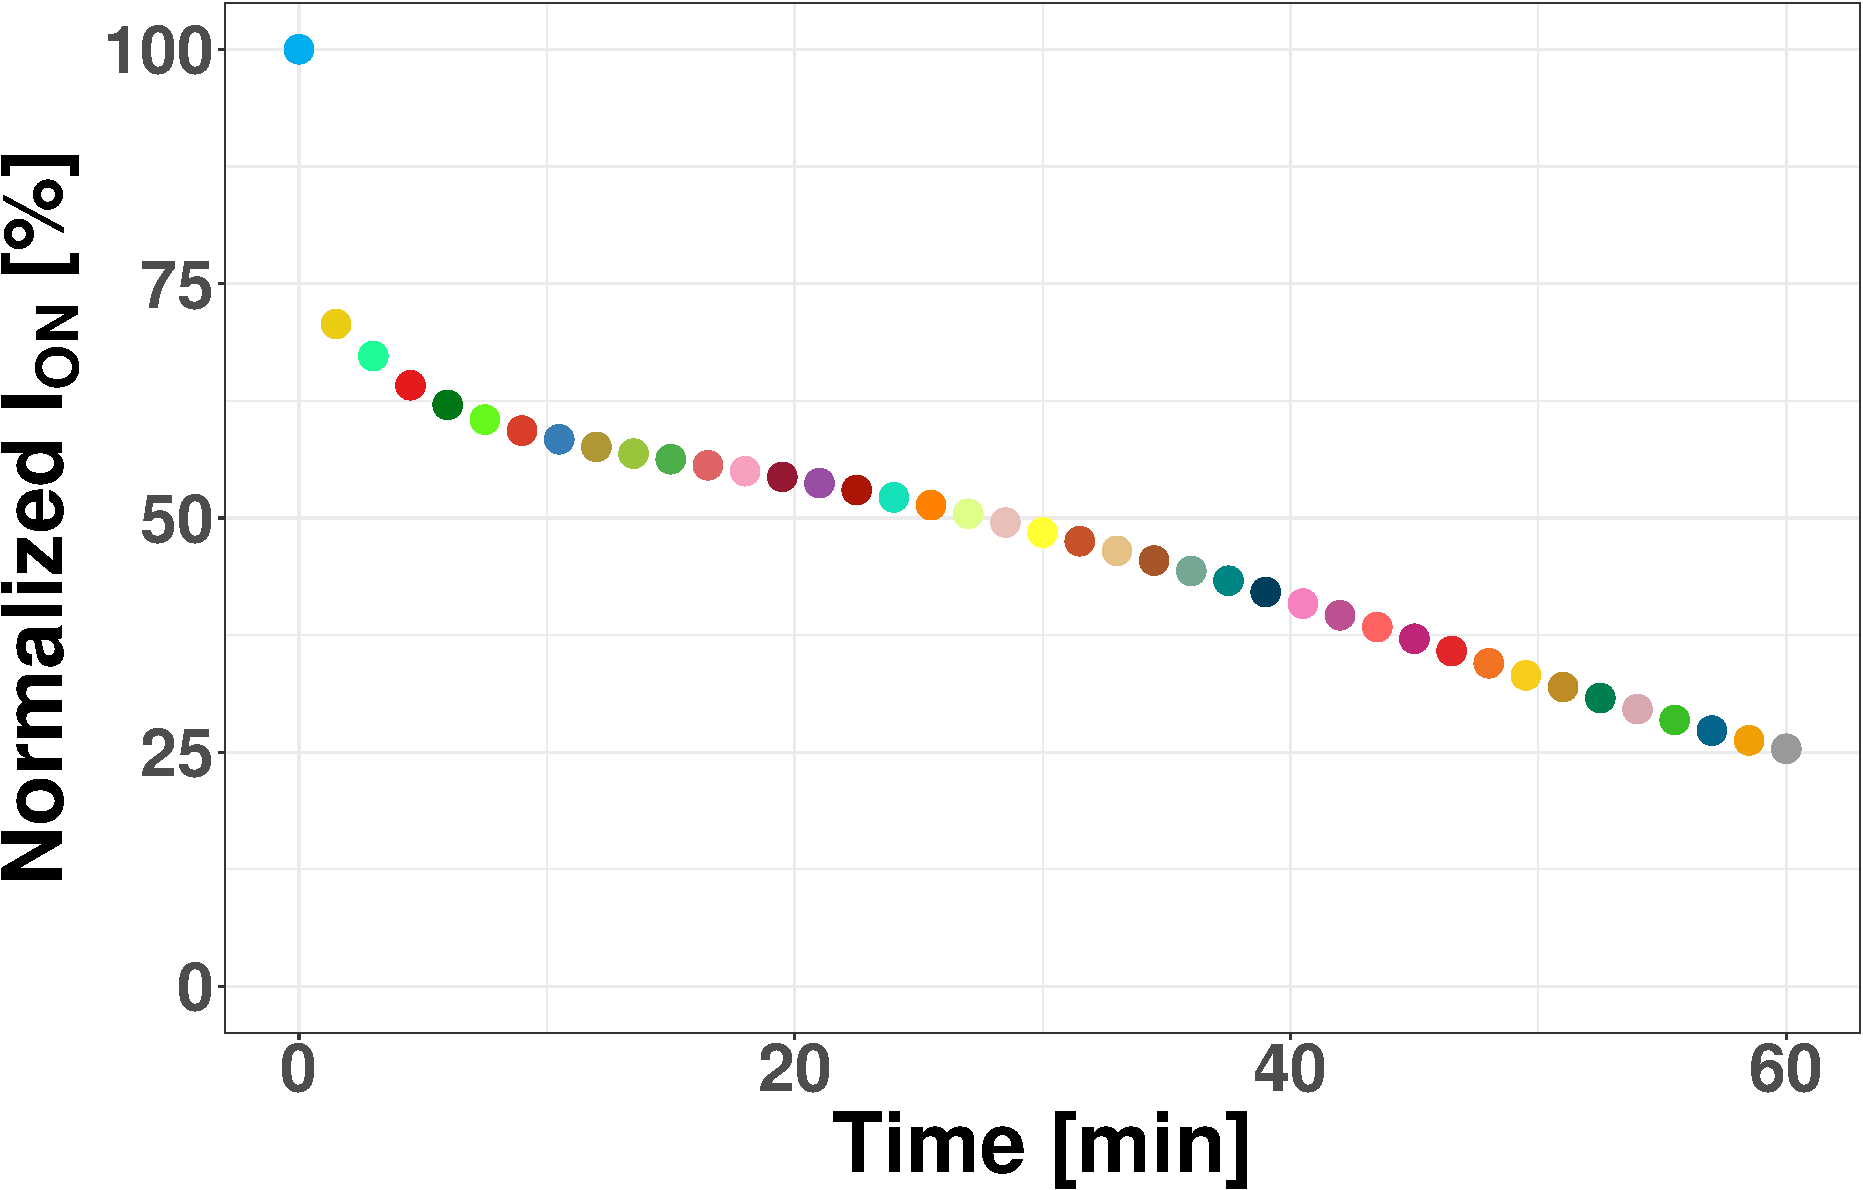
\includegraphics[width=0.45\textwidth]{figures/chapter3/EGFET/NormNoMem.pdf}%
        \label{fig:NormNoMem}
    }
    \caption{Electrical characterization of a standard EG-CNTFET device. 
    (a) The consecutive transfer curves collected over the span of \SI{60}{\min} show that the current decreases prograssively after each measurement, as indicated by the arrow.
    (b) The normalized \ion{} for the same device better highlights the phenomenon of decreasing current, indicating device instability. It is important to note that this instability may compromise the reliability of the platform when used for longer times, as it happens for sensing applications.}
    \label{fig:noMem}
\end{figure}

\begin{figure}
    \centering
    \subfloat[\igs{} and \ids{}]{%
        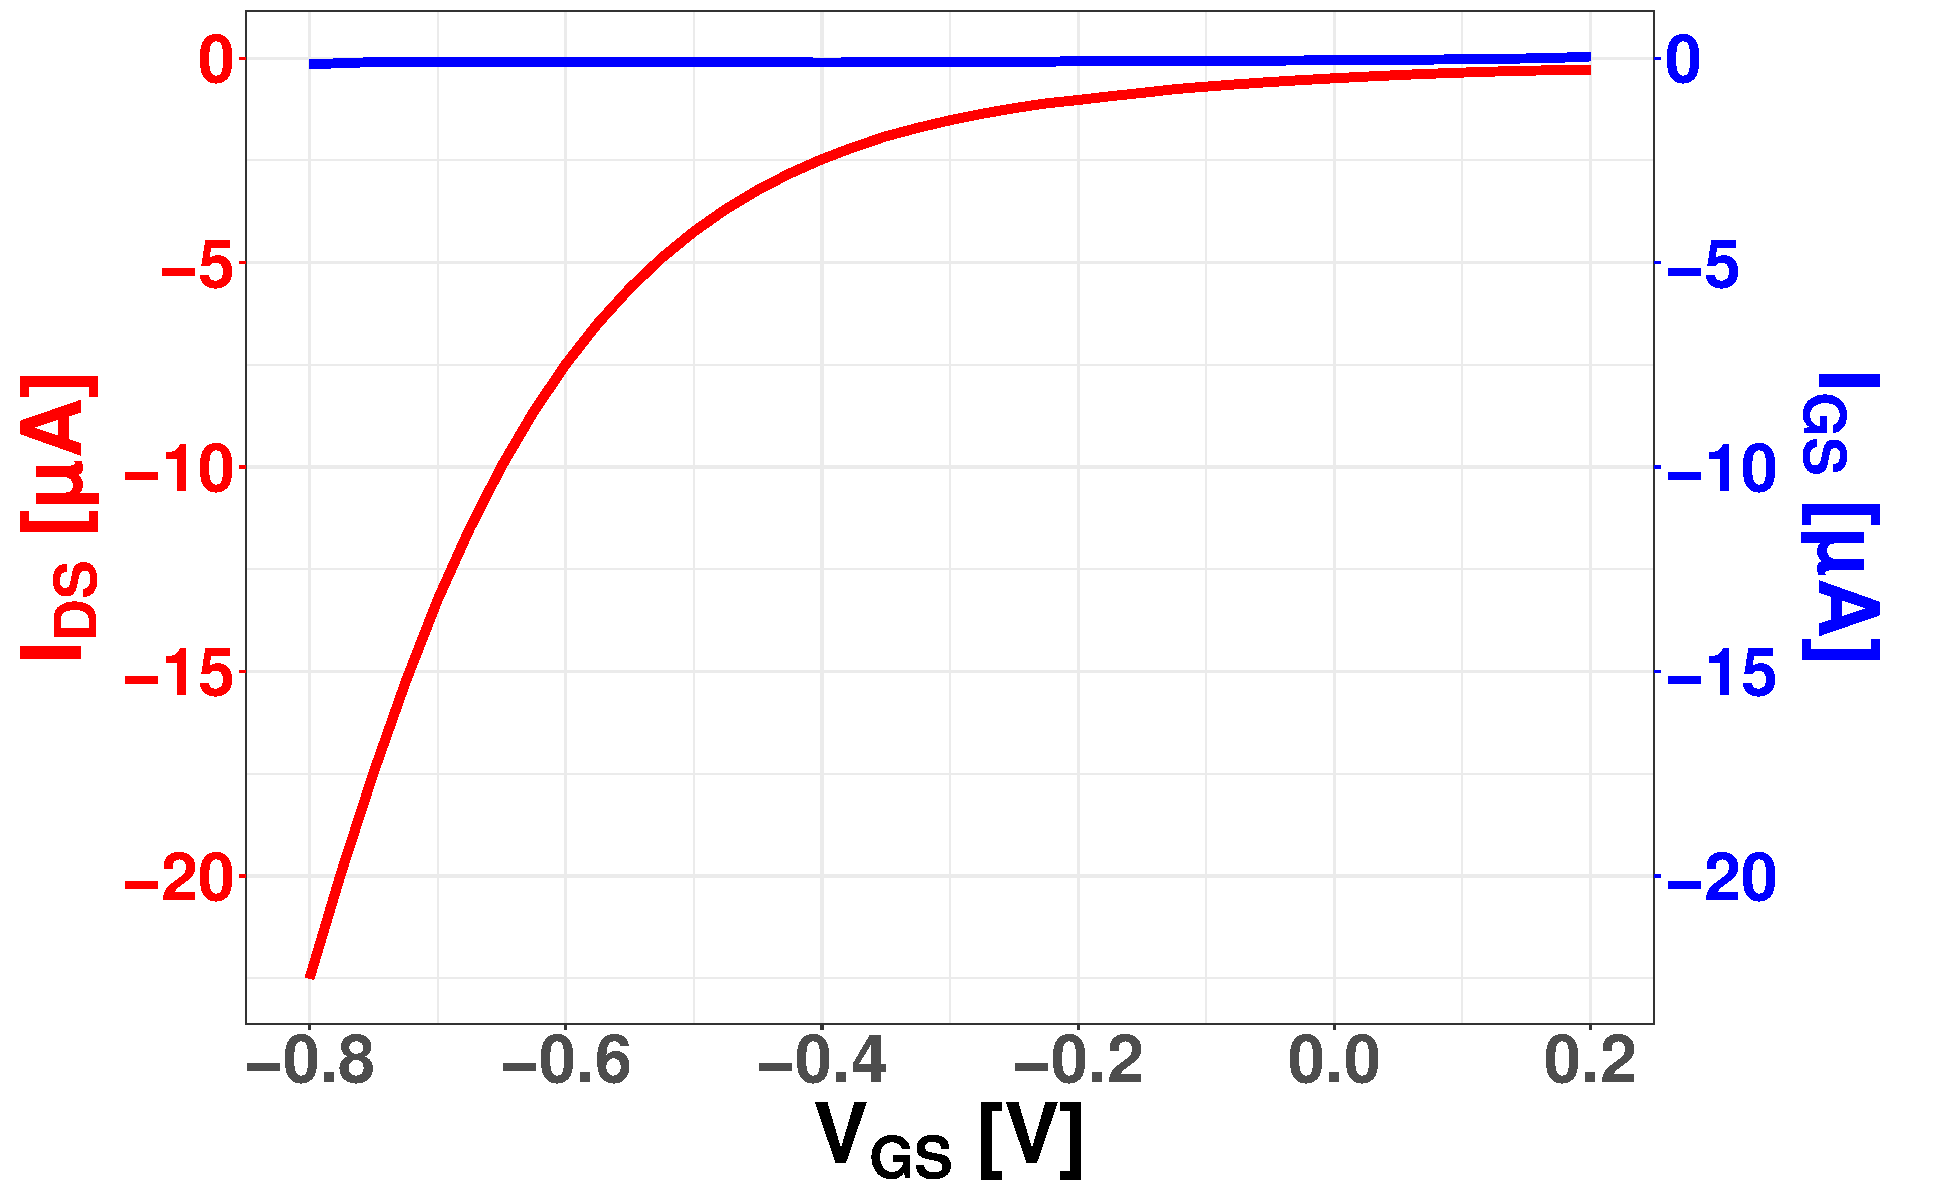
\includegraphics[width=0.45\textwidth]{figures/chapter3/EGFET/IdIgNoMem.pdf}%
        \label{fig:IdIgNoMem}
    }
    \quad
    \subfloat[Hysteresis]{%
        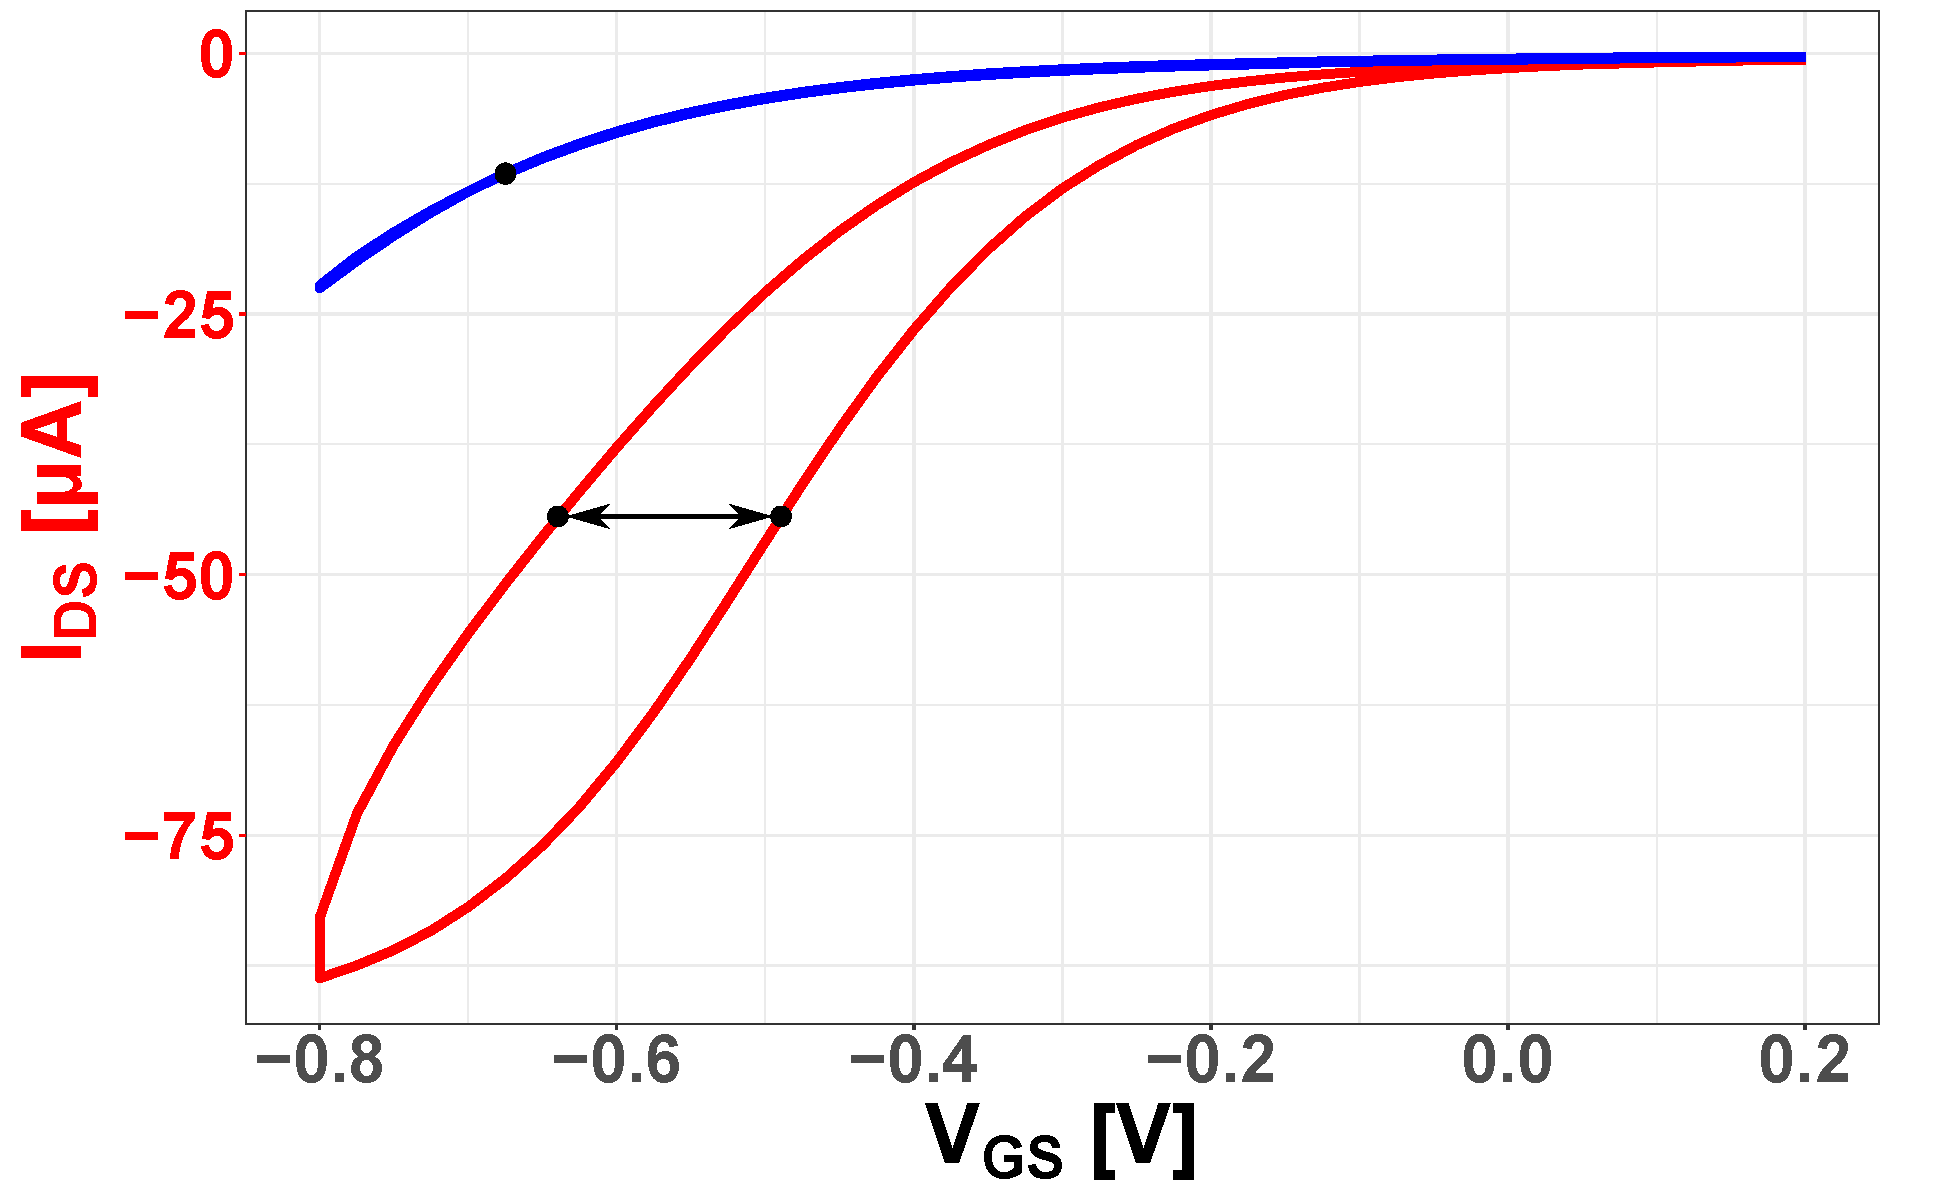
\includegraphics[width=0.45\textwidth]{figures/chapter3/EGFET/hysNoMem.pdf}%
        \label{fig:hysNoMem}
    }
    \caption{Further electrical characterization of the EG-CNTFET devices. 
    (a) Gate current (\igs{}) and drain current (\ids{}): \igs{} is several orders of magnitude lower than \ids{}, indicating low gate leakage. This suggests efficient gate control, reduced power dissipation, and minimized unintended electrochemical reactions at the gate interface, all of which contribute to improved device performance and longevity. 
    (b) Hysteresis decreases greatly from the first (red curve) to the last transfer curve (blue curve), indicating a more stable operation over time.}
    \label{fig:parameters_noMem}
\end{figure}

Figure \ref{fig:IdIgNoMem} shows \ids{} and \igs{} on the same plot: \igs{} is orders of magnitude lower than \ids{}, indicating minimal gate leakage, which is crucial for efficient transistor functioning. Indeed, gate leakage is a phenomenon that occurs when a current flows between the gate and the channel, exiting the designated source-drain path, leading to increased power dissipation, and reduced device efficiency and stability.

Another parameter to consider in device performance is hysteresis, which is defined as \vv{the difference of the voltages that should be applied to the gate in forward and backwards sweeps to get the drain current equal to the average of maximum and minimum drain current, \ie{} ($\frac{I_{\text{D,max}} + I_{\text{D,min}}}{2}$)} \citep{joshiUnderstanding2018}. Several factors contribute to hysteresis, including adsorbed water and oxygen molecules on the CNT surface, and surface traps that capture induced charges \citep{joshiUnderstanding2018,zaumseilSemiconducting2019}. Hysteresis is an important parameter to evaluate, as it can significantly impact device performance: indeed it can affect mobility, threshold voltage, on/off ratio, and sub-threshold slope, potentially causing signal drift and negatively impacting reliability \citep{joshiUnderstanding2018,noyceElectronic2019}.

As shown in Figure \ref{fig:hysNoMem}, hysteresis in the devices herein presented significantly decreases over time, indicating that device performance improves over time. However, it is important to observe that this reduction in hysteresis is concomitant with a decrease in \ids{} that cannot be overlooked.

\begin{figure}[ht]
    \centering
    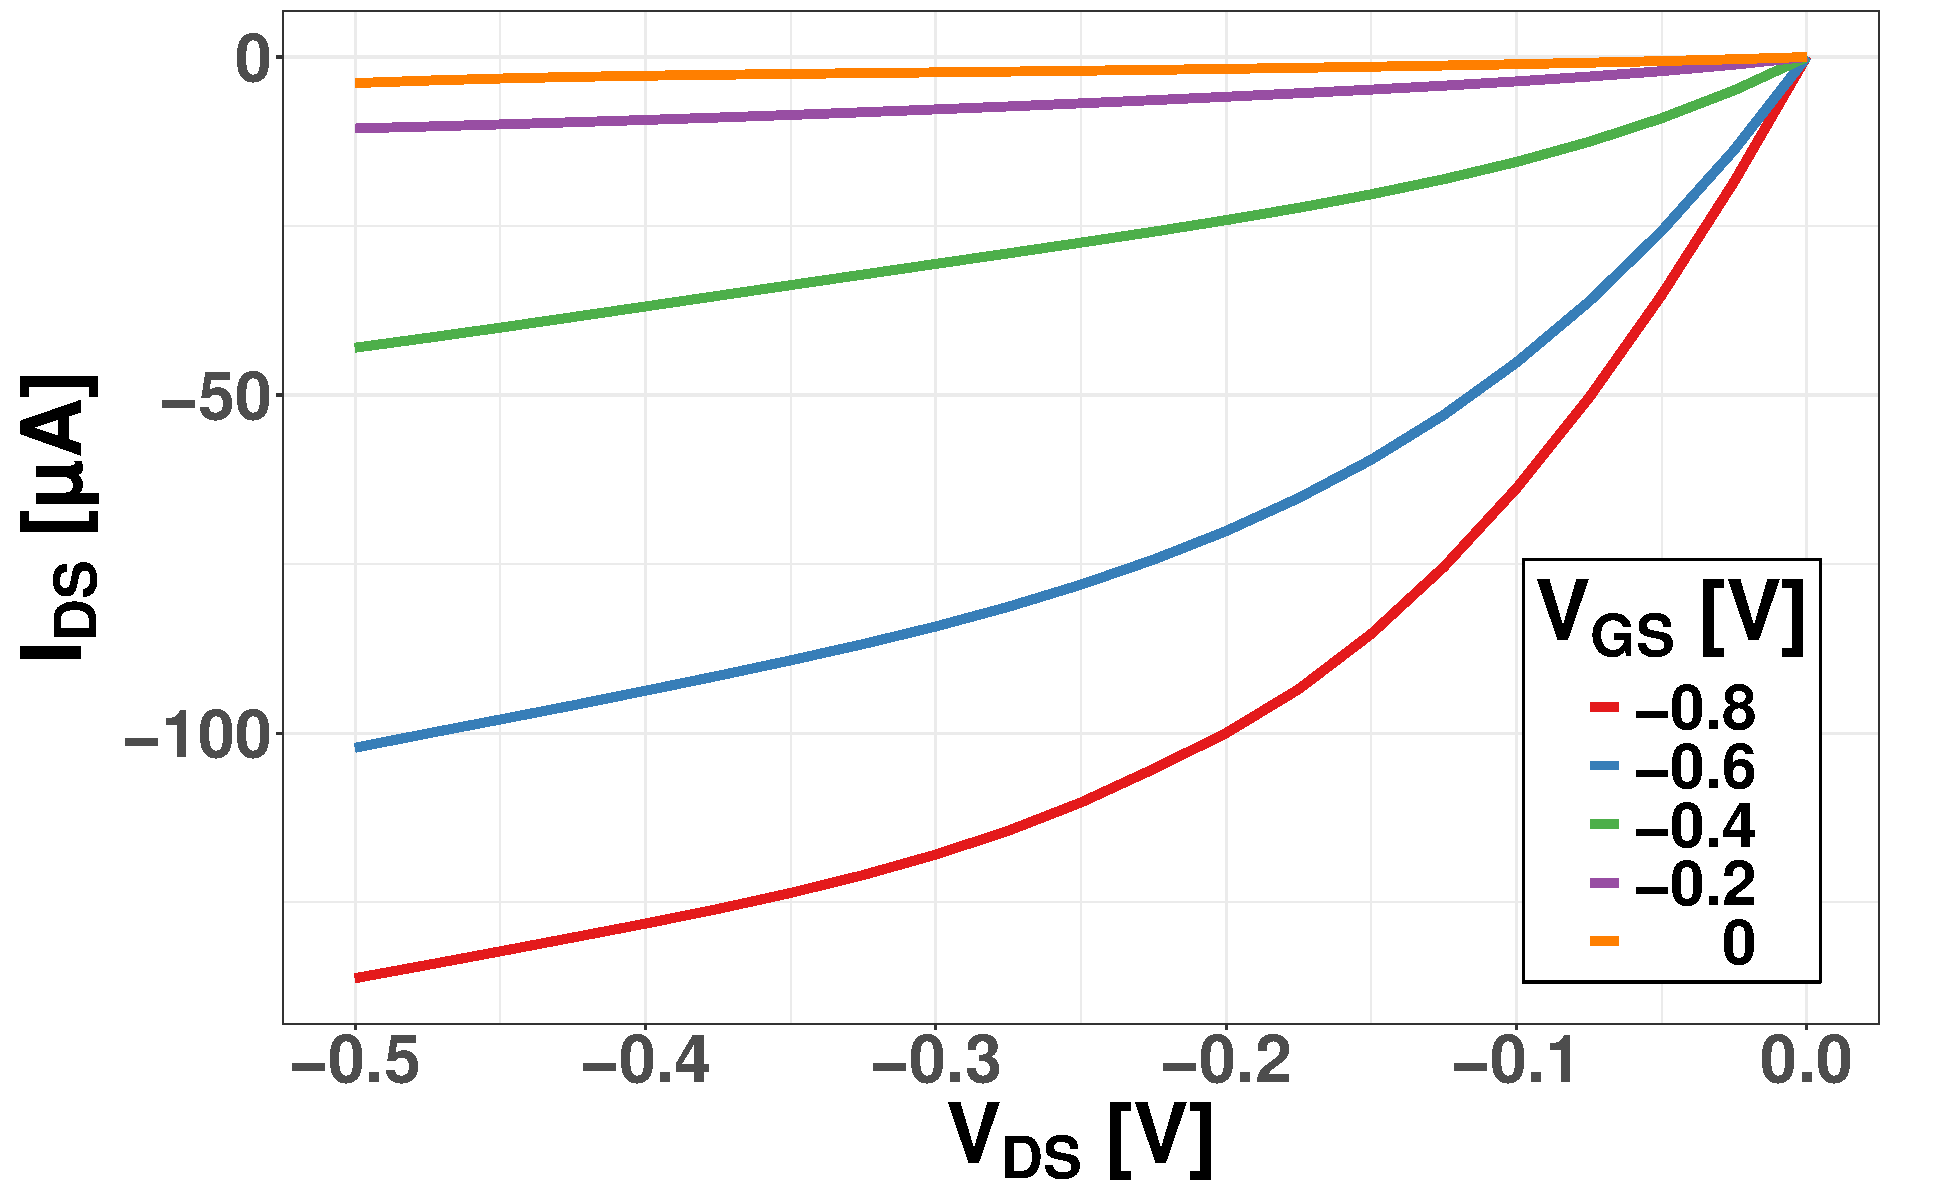
\includegraphics[width=0.45\textwidth]{figures/chapter3/EGFET/outputNoMem.pdf}
    \caption{Electrical characterization of a standard EG-CNTFET device. Output characteristics: the device operates in the linear regime for all \vds{}, although it approaches saturation at \SI{-0.6}{\V} and \SI{-0.8}{\V}. This is supported by the approximately linear trend, which precisely suggests operation in the ohmic region, indicating low contact resistance and efficient charge injection. The well-defined current modulation across different \vgs{} values demonstrates effective gate control, which is essential for stable transistor operation and reliable switching behavior.}
    \label{fig:outputNoMem}
\end{figure}

After the transfer curves, output characteristics were plotted and evaluated (Figure \ref{fig:outputNoMem}): output characteristics describe the relationship between \ids{} and \vds{} for different \vgs{}. By collecting output characteristics, it is possible to further assess device performance by extrapolating other parameters; in particular, observing these curves allowes to evaluate whether a device operates in linear or saturation regime. Indeed, from the curves displayed in Figure \ref{fig:outputNoMem}, it is possible to gather that the devices approach saturation but do not fully reach it. In fact, in a well-saturated regime, \ids{} would become relatively constant with increasing \vds{}; the incomplete saturation seen in these devices suggests that there may be residual channel conduction even at high \vds{}, due to factors such as inefficient carrier pinch-off, contact resistance, or electrostatic limitations of the electrolyte gating mechanism.

\subsection{Membrane encapsulation}
\label{sec:membrane_encapsulation}

With a baseline established, it is evident that the devices are not stable over time, as demonstrated by the decreasing current over time. The objective of this project was to develop an inexpensive approach to improve device stability while also achieving faster stabilization. To tackle this issue, a lipophilic membrane was deposited on the CNTs of the channel to protect them from environmental exposure. Indeed, CNTs degrade upon contact with the oxygen in the air and with the water molecules of the electrolyte, causing an alteration in device performance. Great care must be therefore given to these devices, to the point that they must be stored in a protected environment, \ie{} a nitrogen-filled glovebox, to prevent damages to the nanotubes in the time prior to the measurements. Additionally, during the measurements, CNTs are exposed to the ions contained in the electrolyte, which could react with the functional groups on the nanotubes and thus further contribute to the worsening performance.

The first step in this approach was optimizing the membrane deposition process itself, \ie{} the volume to be dropcast and the resulting membrane thickness. Initially, \SI{10}{\ul} of the membrane were dropcasted onto the CNT channel in a one-step deposition. This proved insufficient in providing consistent protection: 50\% of devices reached higher stability (Figure \ref{fig:norm10bad}), while the other half still exhibited worsening behaviour during measurements (Figure \ref{fig:norm10bad}), indicating that the CNTs were still suffering the consequences of air and electrolyte exposure ($N = 12$). Given this variability, an alternative deposition strategy needed to be developed to ensure a more reliable coverage.

\begin{figure}
    \centering
    \subfloat[Normalized \ids{} of a device that does not stabilize]{
        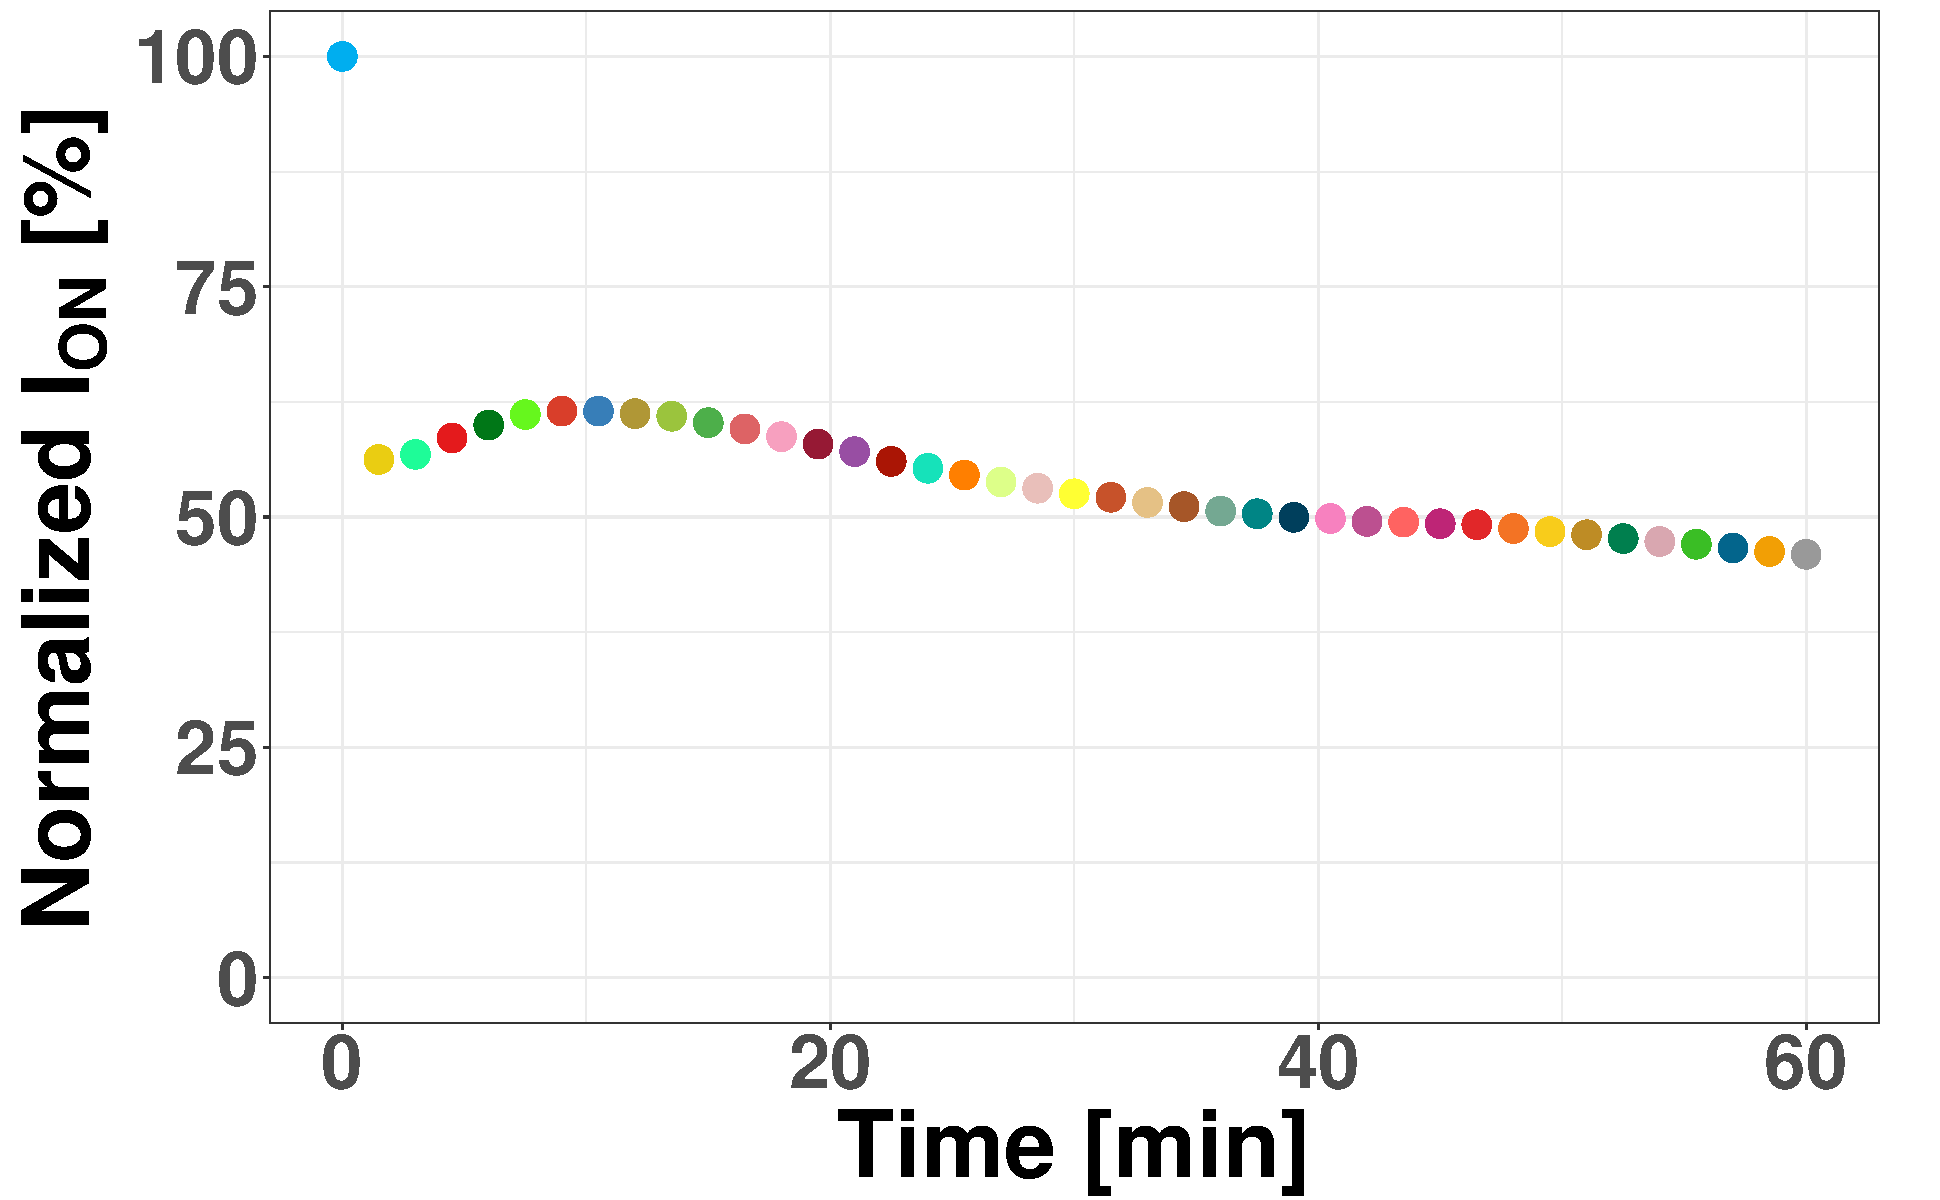
\includegraphics[width = 0.45\textwidth]{figures/chapter3/EGFET/norm_bad.pdf}
        \label{fig:norm10bad}}
    \subfloat[Normalized \ids{} of a device that does stabilize]{
        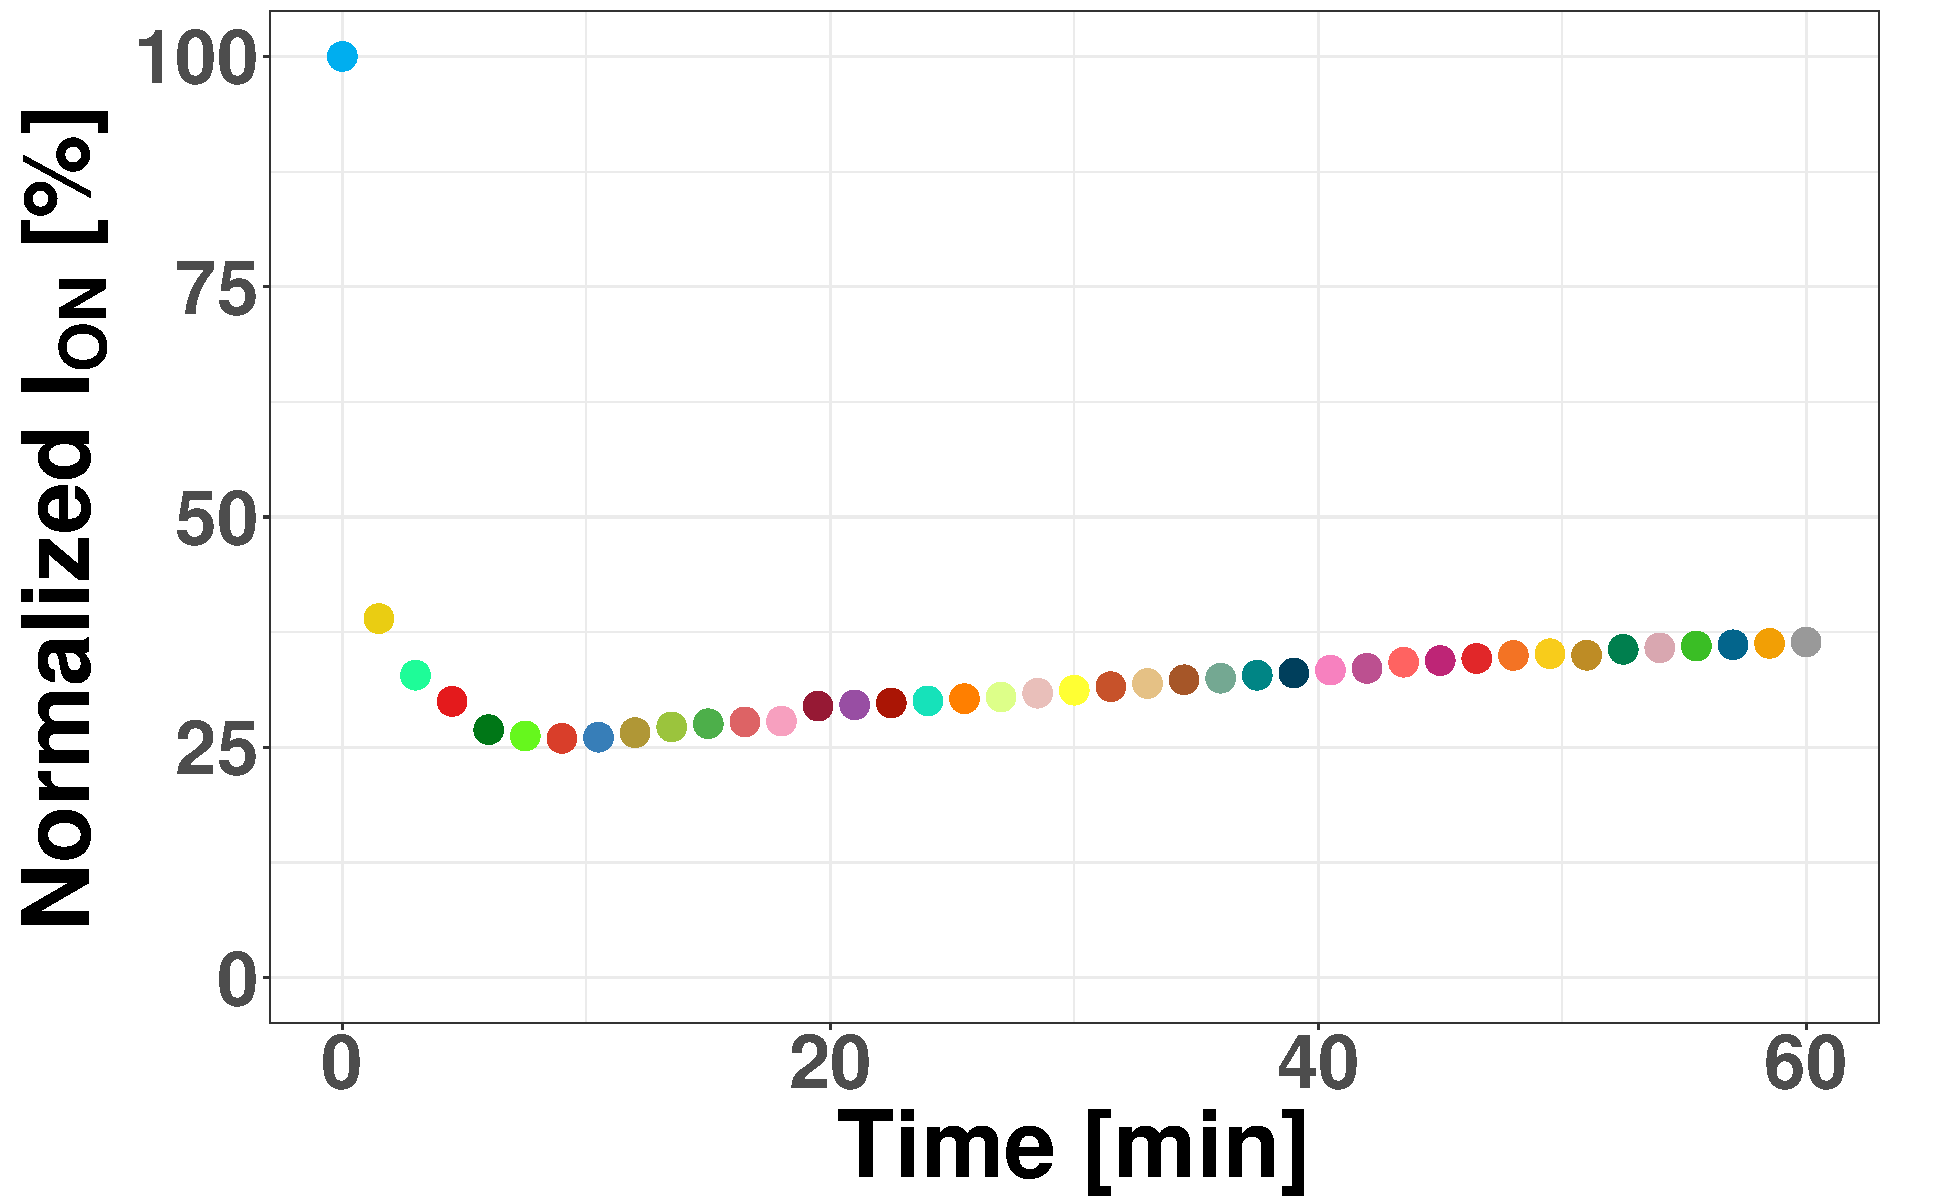
\includegraphics[width = 0.45\textwidth]{figures/chapter3/EGFET/norm_good.pdf}
        \label{fig:norm10good}}
    \caption{
        Comparison of the normalized \ids{} of two EG-CNTFETs with \SI{10}{\micro\l} of lipophilic membrane dropcasted on the channel. The results show mixed behaviour: 
        (a) 50\% of the devices display a similar behaviour to the EG-CNTFETs with the bare channel, indicating that the membrane does not provide protection from the environment.
        (b) 50\% of the devices stabilize over time, as indicated by the increasing current. The results were not satisfactory and more work needed to be done to provide full CNT protection.}
    \label{fig:membrane10ul}
\end{figure}

It was found that a two-step dropcasting process, \ie{} first depositing \SI{8}{\ul} and following with an additional \SI{7}{\ul}, resulted in effective CNT coverage while still allowing current to flow.
First, the change in \rds{} before and after membrane deposition was tested, as demonstrated by Figure \ref{fig:rdsChange}. The expected result was an increase, due to the lower ion content of the membrane and to the addition of scattering centers in the channel \citep{joshiUnderstanding2018}. The measurements confirmed the expectations, showing a value of \SI{2.25}{} $\pm$ \SI{0.94}{\kohm} on the bare channel (before membrane deposition), while the \rds{} increased to \SI{24.48}{} $\pm$ \SI{8.45}{\kohm} with the membrane protecting the SWCNT network. The result is also consistent with the findings of \citet{petrelliMethod2023}, who observed an approximately 15-fold increase in resistance after the deposition of an ion-selective membrane on the channel, also accompanied by an increase in variability.

\begin{figure}
    \centering
    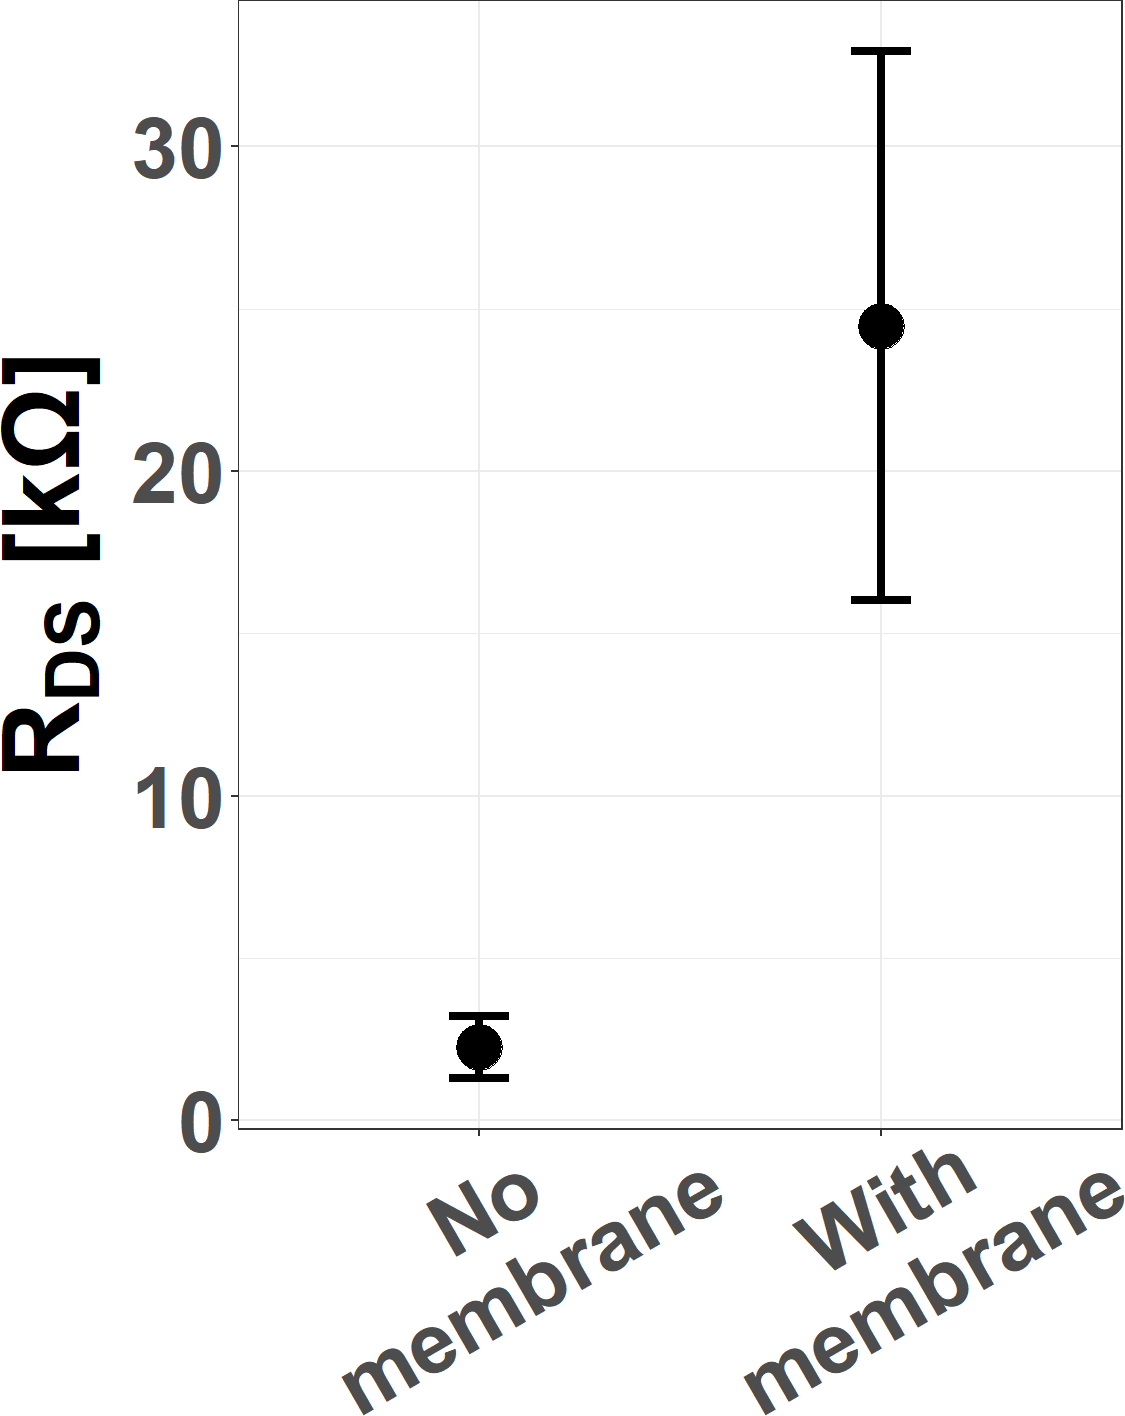
\includegraphics[width = 0.3\textwidth]{figures/chapter3/EGFET/Rds_change.png}
    \caption{Variation in resistance between source and drain (\rds{}) before and after the deposition of the lipophilic membrane. Before membrane deposition, the devices exhibit a resistance of \SI{2.25}{} $\pm$ \SI{0.94}{\kohm}, with little variability among them; this is thanks to the previous screening that was carried out for the purpose of having the best performing platforms, while also reducing device-to-device variation. After membrane deposition, the resistance increases, together with the standard deviation, indicating greater variability among the devices.}
    \label{fig:rdsChange}
\end{figure}

\begin{figure}
    \centering
    \subfloat[Transfer characteristics]{%
        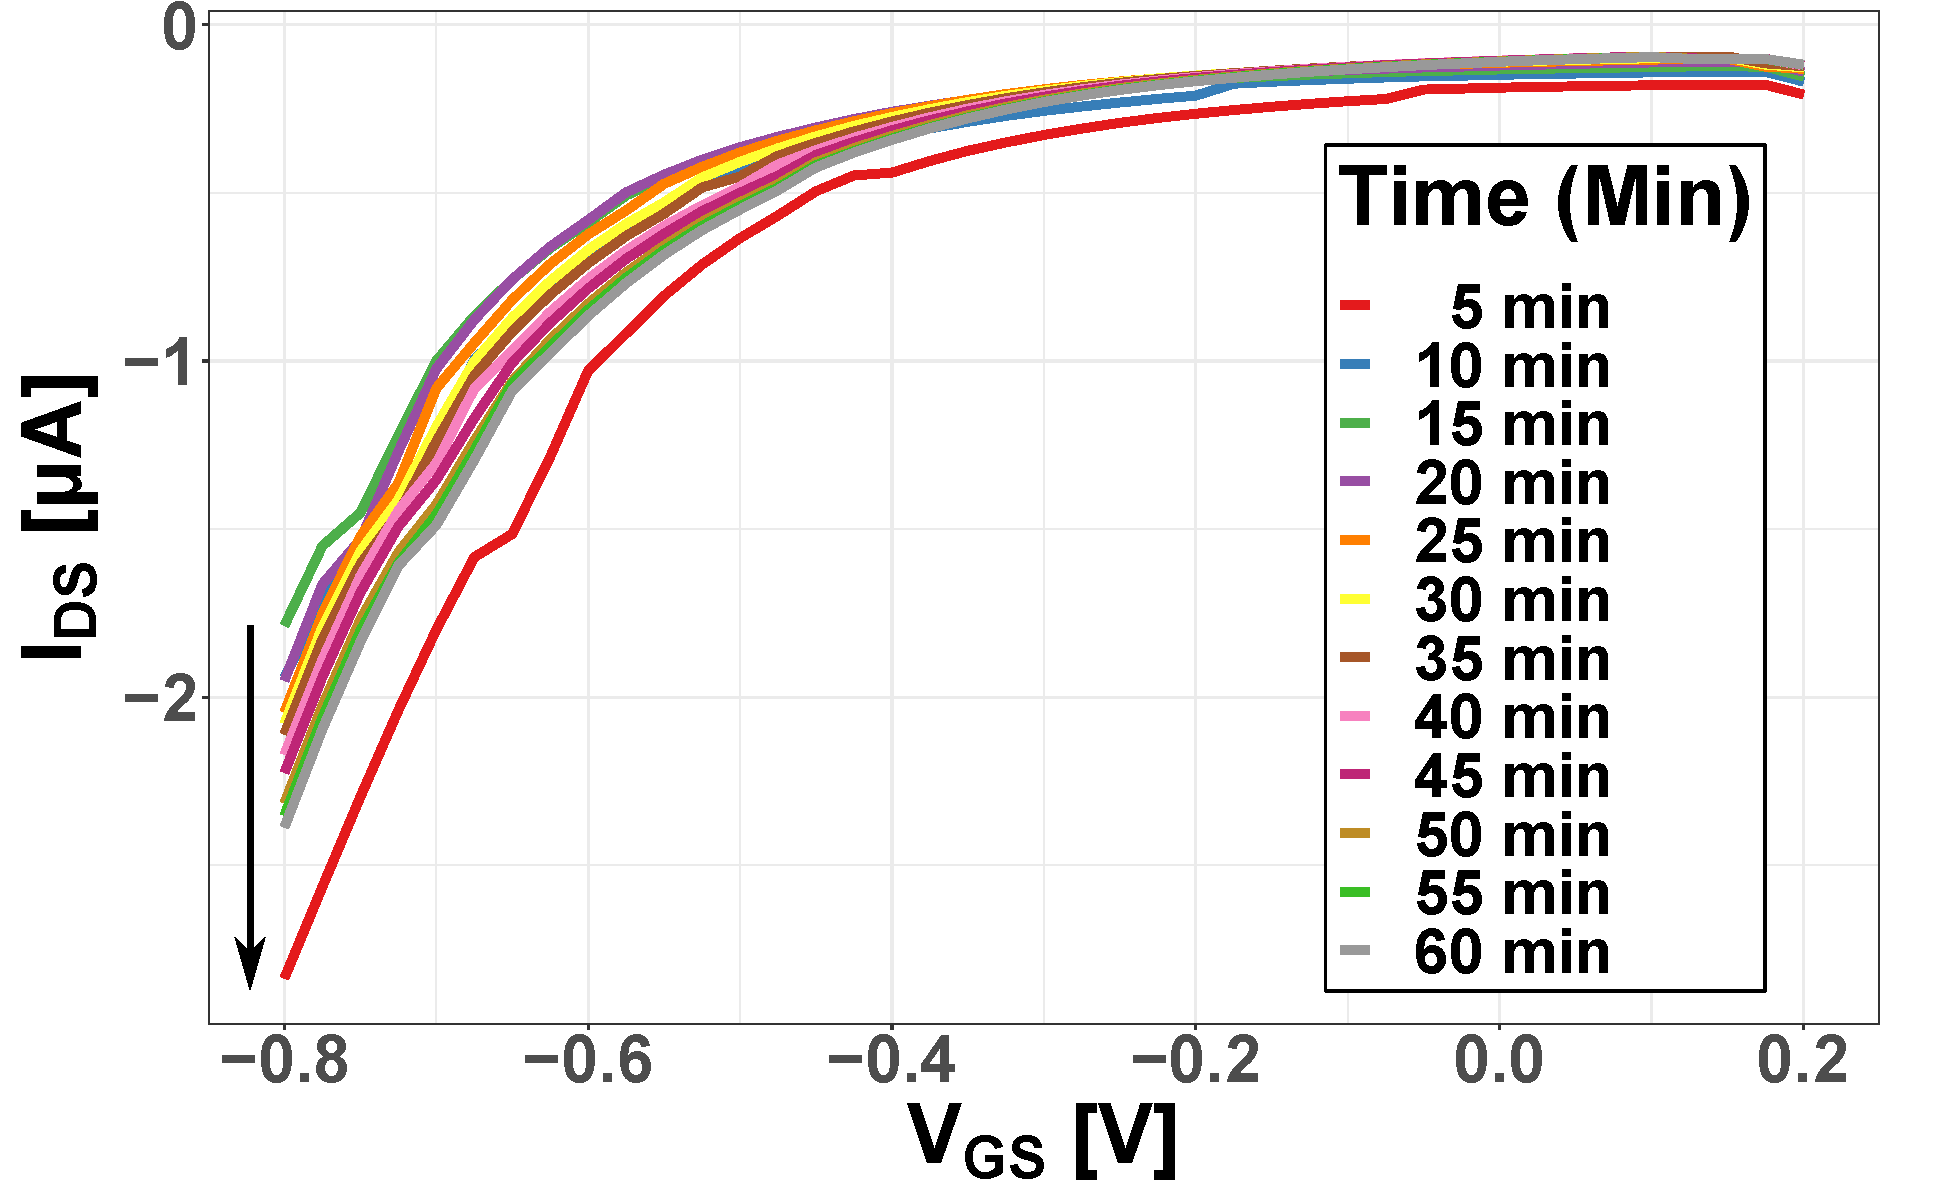
\includegraphics[width=0.45\textwidth]{figures/chapter3/EGFET/transferMem.pdf}%
        \label{fig:transferMem}
    }
    \quad
    \subfloat[Normalized \ion{}]{%
        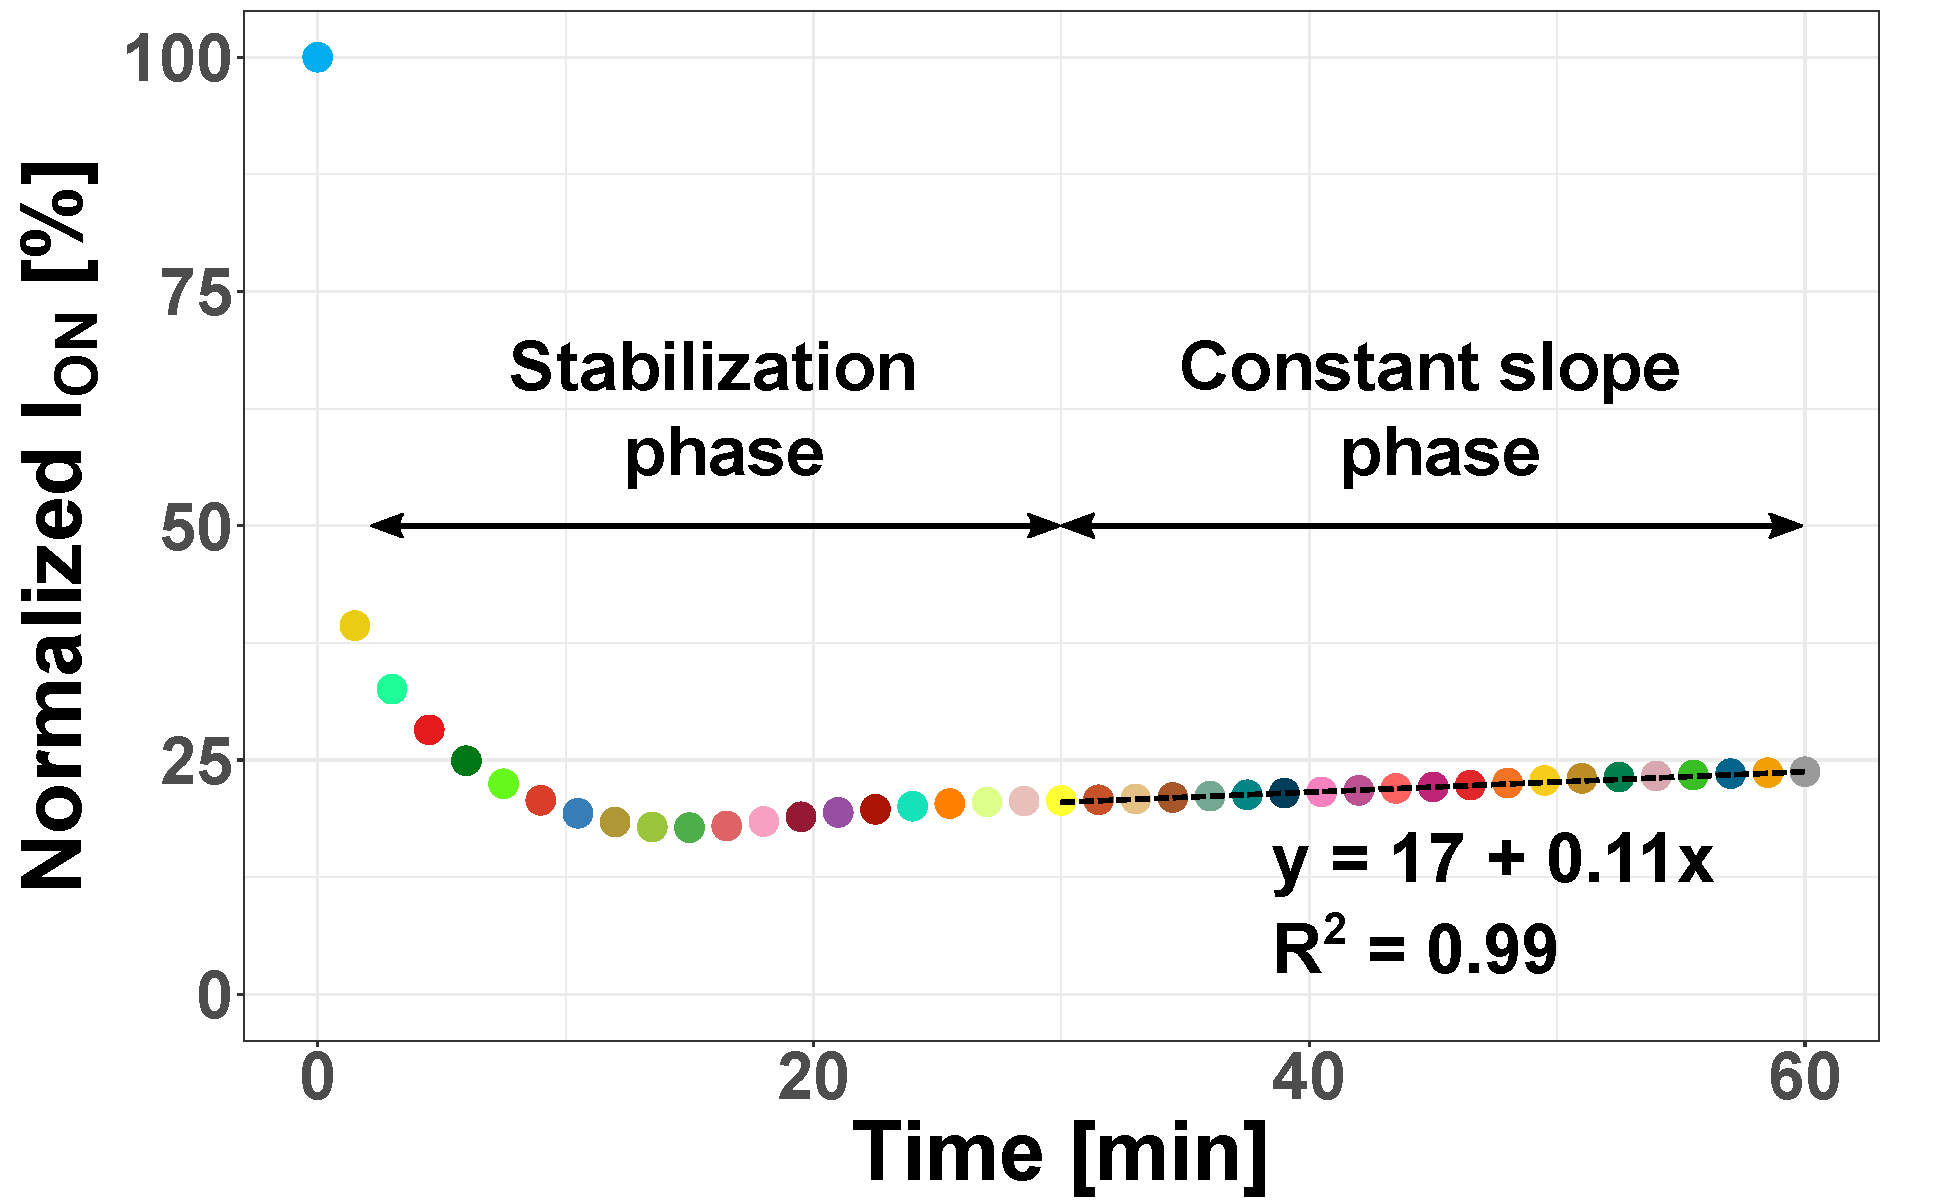
\includegraphics[width=0.45\textwidth]{figures/chapter3/EGFET/NormMem.pdf}%
        \label{fig:normMem}
    }
    \caption{
        Electrical characterization of an EG-CNTFET device with a lipophilic membrane on the channel (\SI{8}+\SI{7}{\micro\l}). 
        (a) The transfer characteristics show an increasing current over time.
        (b) The normalized \ion{} better displays the current increase and allows to distinguish two phases: first, the \emph{stabilization phase}, where the EDLs are still forming and an equilibrium must be found, then the \emph{costant slope phase}, where the current becomes linear with respect to time.}
    \label{fig:Mem}
\end{figure}

The transfer curves of the devices with an encapsulated channel, shown in Figure \ref{fig:transferMem}, exhibit a different trend compared to the unencapsulated counterparts (Figure \ref{fig:transferNoMem}). The first transfer curve, collected five minutes after the start, shows the highest current, however, it is possible to observe that the other curves are plotted at lower values, then progrssively increasing again over time. This current evolution is again better visualized through the normalized \ids{}, as seen in Figure \ref{fig:normMem}. Two distinct phases in the device behavior can be distinguished: the initial phase can be referred to as the \emph{stabilization phase}, lasting approximately the first \SI{30}{\min}. During this period, the electrical double layers (EDLs) are still forming, ions are moving and potentially being trapped in the membrane, and the system is moving toward an equilibrium. This is hypothesized from the fact that, after the first point, the current decreases by more than half and exhibits significant variability, without following a specific trend. Following the stabilization phase, the system enters the so-called \emph{constant slope phase}, where the \ion{} displays a linear trend over time; for the scope of this analysis, the trend was considered linear for $R^2>0.98$. On average, the devices achieved this linearity in \SI{33.8}{} $\pm$ \SI{12.9}{\min}, effectively halving the stabilization time compared to state-of-the-art devices \citep{molazemhosseiniRapidly2021}. This stabilization is particularly relevant for EG-CNTFETs employed as transducers in sensor applications: indeed, a linear baseline can be subtracted from the measured current during analyte detection, improving measurement reliability. This leads to accurate platform calibration, ultimately allowing precise quantification of analytes in samples.

It is important to notice that, the current is now an order of magnitude lower than that of the bare devices. However, this reduction is not a major concern, as the signal remains measurable. This trade-off must be therefore considered when assessing device performance, as a lower yet stable current is preferable to a higher current that decreases rapidly due to semiconductor degradation, ultimately leading to the loss of signal.

\begin{figure}
    \centering
    \subfloat[\igs{} and \ids{}]{%
        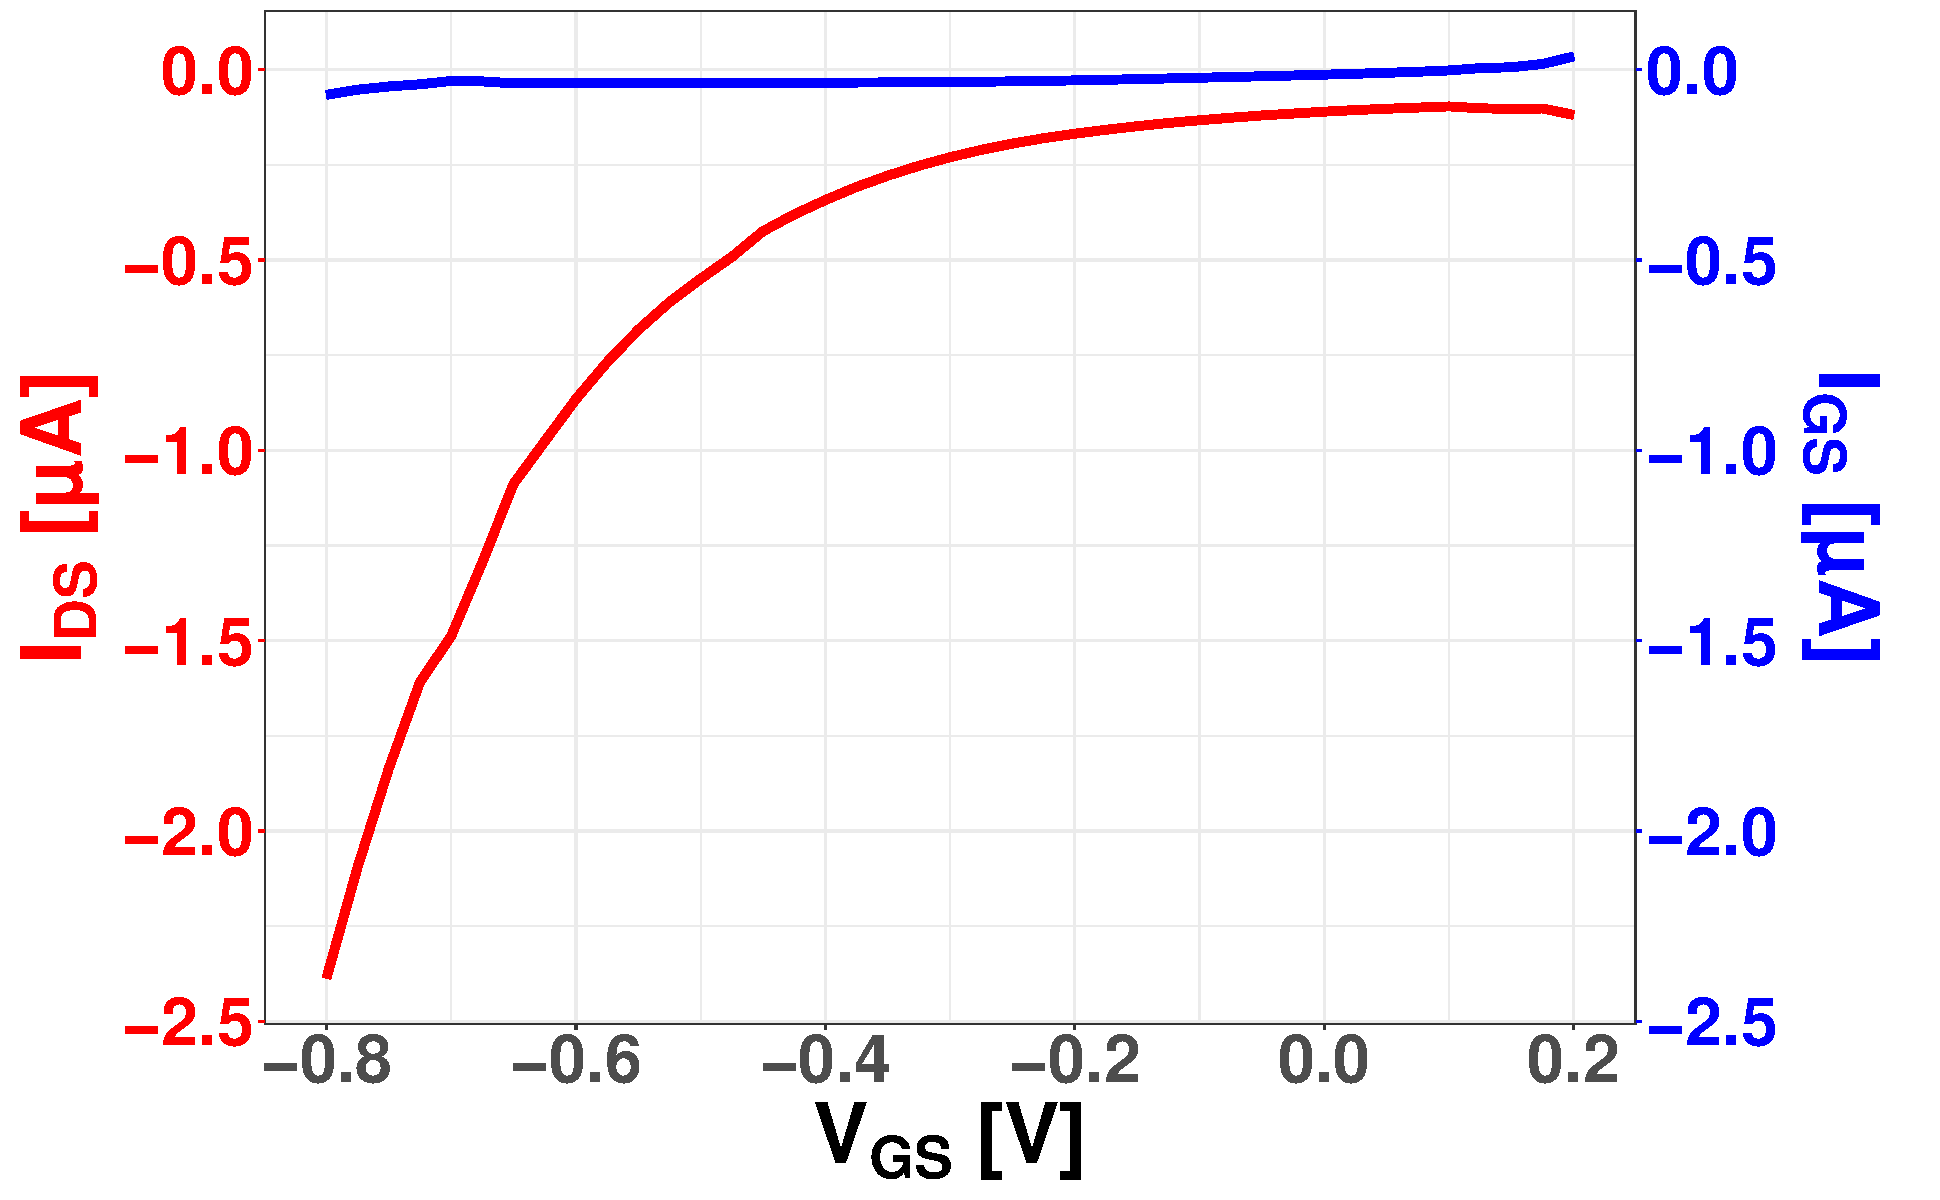
\includegraphics[width=0.45\textwidth]{figures/chapter3/EGFET/IdIgMem.pdf}%
        \label{fig:IdIgMem}
    }
    \quad
    \subfloat[Hysteresis]{%
        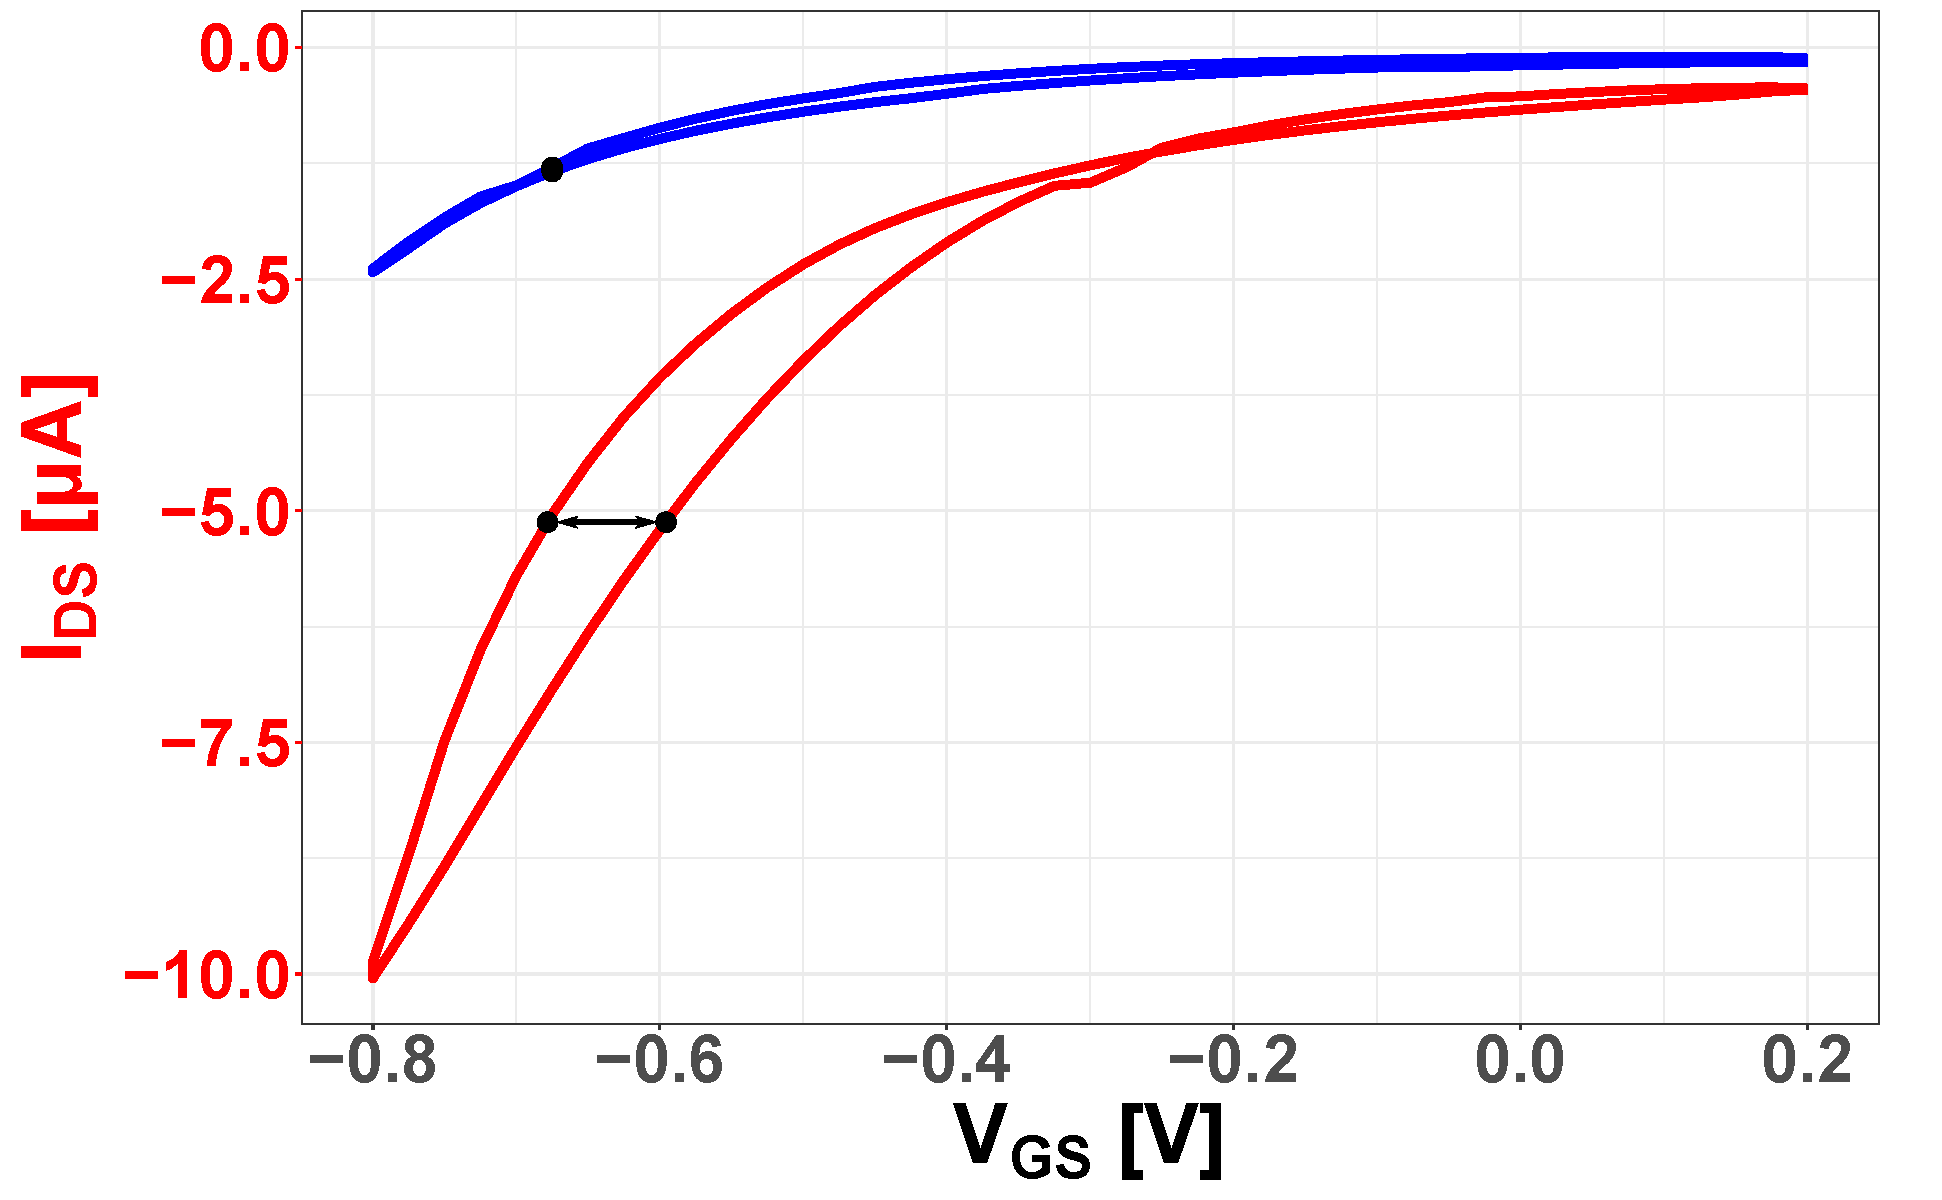
\includegraphics[width=0.45\textwidth]{figures/chapter3/EGFET/hysMem.pdf}%
        \label{fig:hysMem}
    }
    \caption{Further electrical characterization of an EG-CNTFET device with a lipophilic membrane on the channel. 
    (a) Gate current (\igs{}) and drain current (\ids{}): as in the case of the bare channel, \igs{} is several orders of magnitude lower than \ids{}, indicating low gate leakage. 
    (b) Hysteresis: devices with the membrane exhibit reduced hysteresis even at the start of the experiment (red curve), suggesting improved charge stability and reduced trapping effects. It is noteworthy that also in this case, the current decreases significantly from the first transfer recorded to the last (blue curve).}
    \label{fig:parameters_Mem}
\end{figure}

Figure~\ref{fig:parameters_Mem} shows a couple important electrical parameters of the device, \ie{} the \igs{} with respect to the \ids{} (Figure \ref{fig:IdIgMem}) and the hysteresis (Figure \ref{fig:hysMem}). In the first plot, the gate current is two orders of magnitude lower than the drain current; this is the expected outcome, with minimal gate leakage current. The small deviation observed in \igs{} indicates the presence of minor leakage pathways, but their negligible magnitude confirms that the device maintains effective electrostatic control. The right panel illustrates how hysteresis changes from the first (red) to the last (blue) transfer curves collected. Initially, the red curve exhibits a large hysteresis, with the drain current reaching approximately \SI{-10}{\uA}; by the end of the measurement, the current is significantly lower (\SI{-2.5}{\uA}) and the hysteresis now amounts to \SI{0}{\V}. This improvement is the desired outcome, which indicates that the device finds a level of stabilization, likely due to the filling of trap states or improved charge screening effects.

Compared to previous results, the latter device shows an overall reduction in conduction (the current is 10 times lower), and yet an improvement in stability.

\begin{figure}
    \centering
    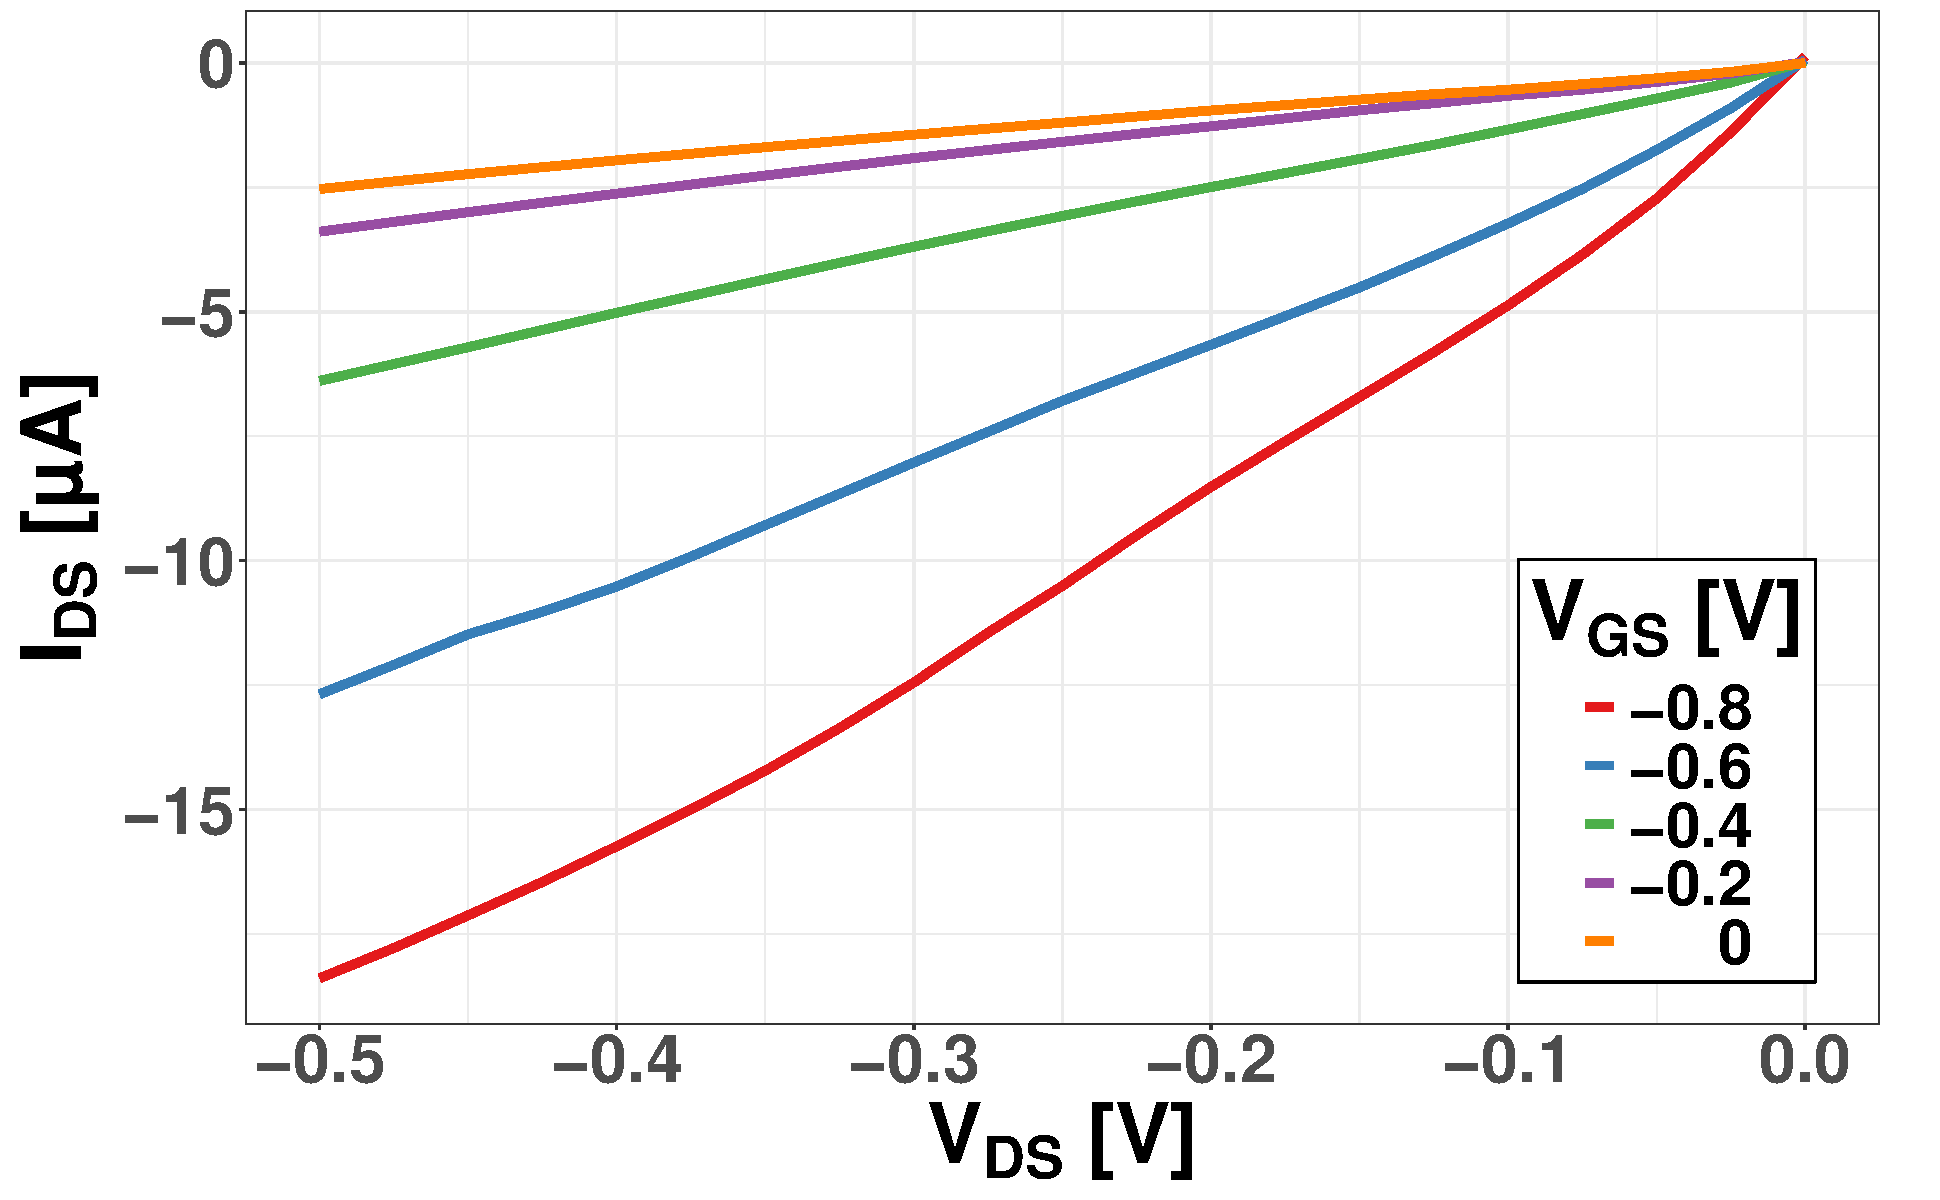
\includegraphics[width=0.45\textwidth]{figures/chapter3/EGFET/outputMem.pdf}
    \caption{Electrical characterization of an EG-CNTFET device with a lipophilic membrane on the channel. Output characteristics: compared to Figure \ref{fig:outputNoMem}, where devices approach saturation, the output curves here indicate that the devices fully remain in linear regime. This suggests that the presence of the membrane affects charge transport and the formation of the accumulation layer, potentially modifying the gating efficiency.}
    \label{fig:outputMem}
\end{figure}

Figure~\ref{fig:outputMem} shows the output characteristics of the device with the channel encapsulated with the lipophilic membrane. Compared to the curves in Figure~\ref{fig:outputNoMem}, there is a notable difference: while the bare devices approached saturation, the encapsulated ones remain far from the saturation regime. This behavior may indicate that the membrane influences charge transport within the channel. The causes could be manifold: for starters, the higher \rds{} due to the membrane limits current injection,  preventing the device from reaching higher current levels and consequently, saturation. For the bare devices, on the other hand, the CNT network is in direct contact with the environment and benefits from more efficient charge injection and transport, leading close to saturation at higher gate voltages. ANother possible explanation is the fact that it is possible that the interaction between the lipophilic membrane and the CNTs alters their electronic properties, negatively influencing the carrier mobility and density, which directly affect current flow, and further contribute to failure to reach saturation.

\begin{figure}
    \centering
    \subfloat[4 hour measurement]{%
        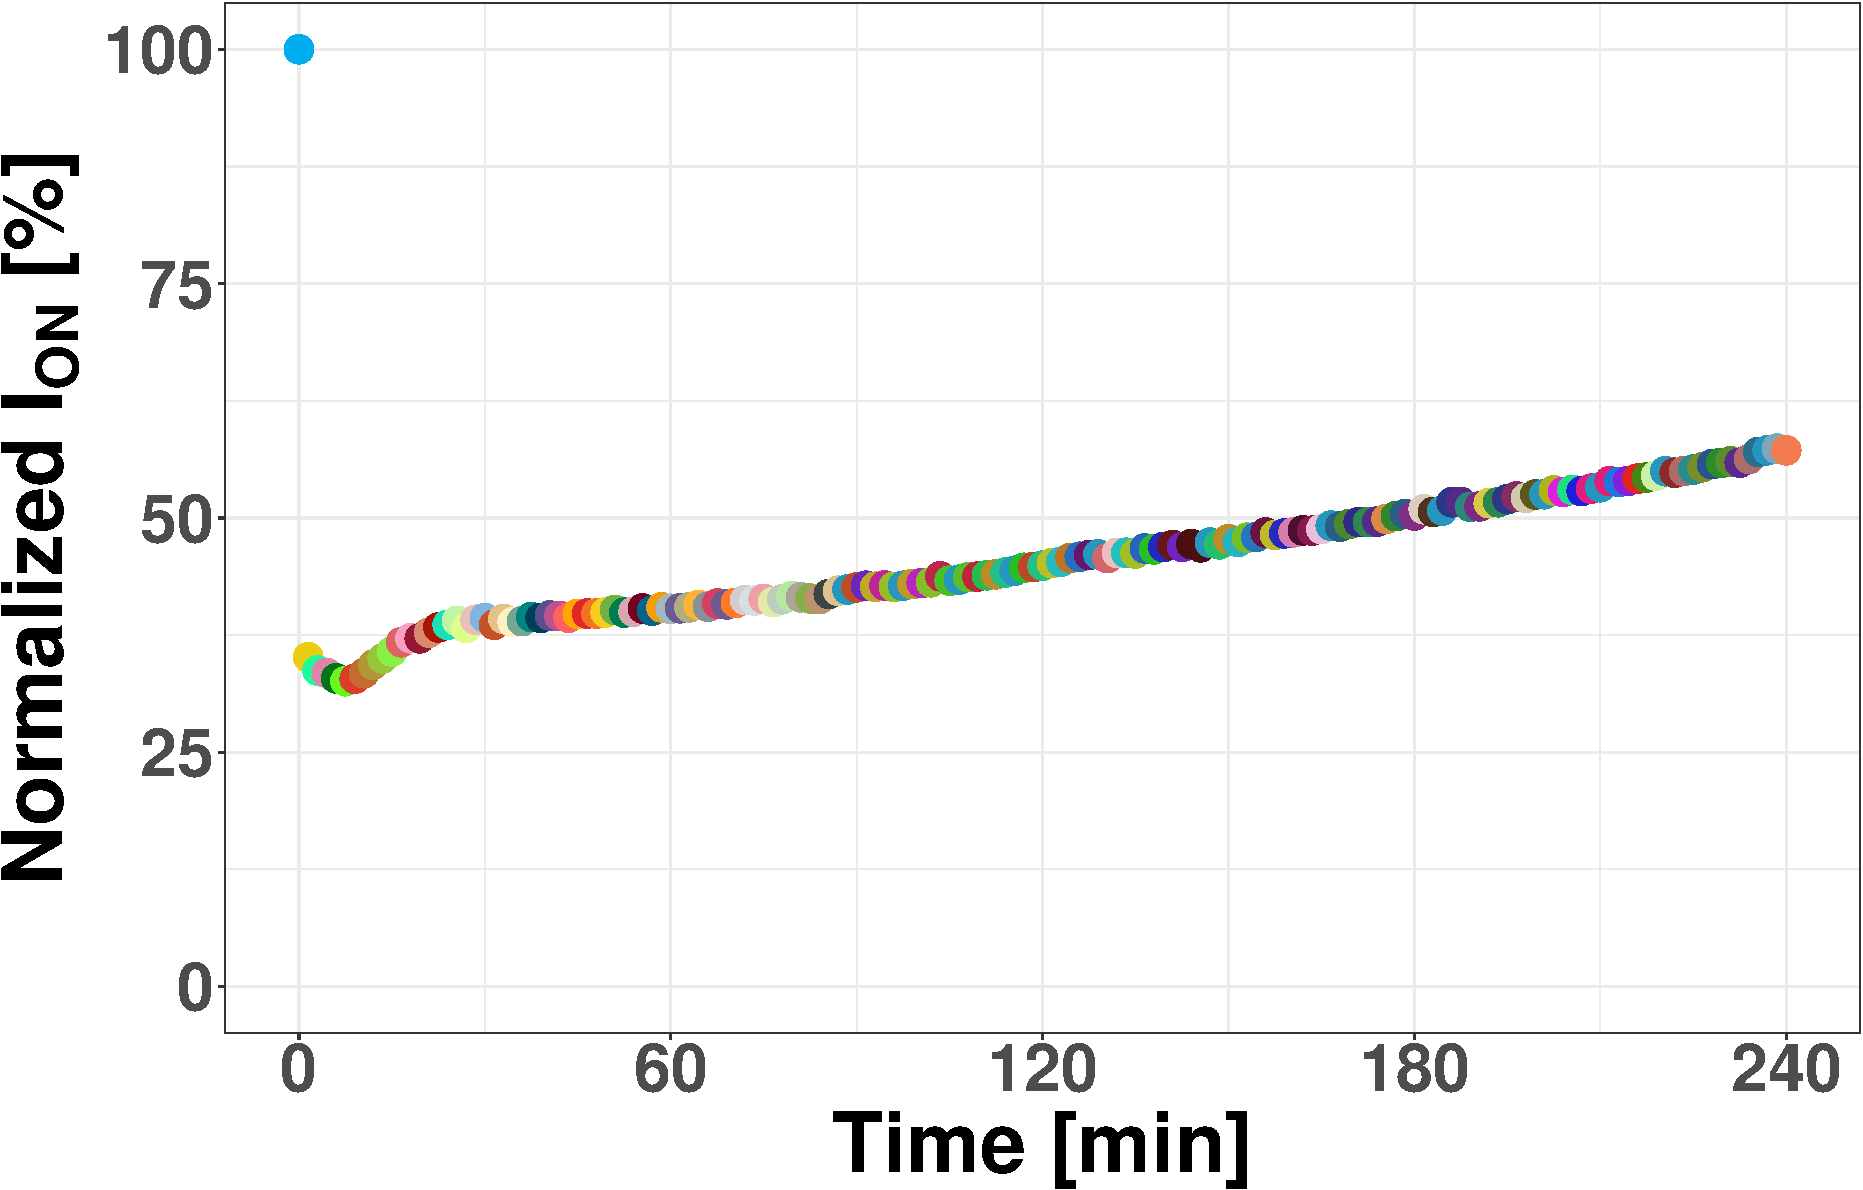
\includegraphics[width=0.45\textwidth]{figures/chapter3/EGFET/norm4h.pdf}%
        \label{fig:norm4h}
    }
    \quad
    \subfloat[12 hour measurement]{%
        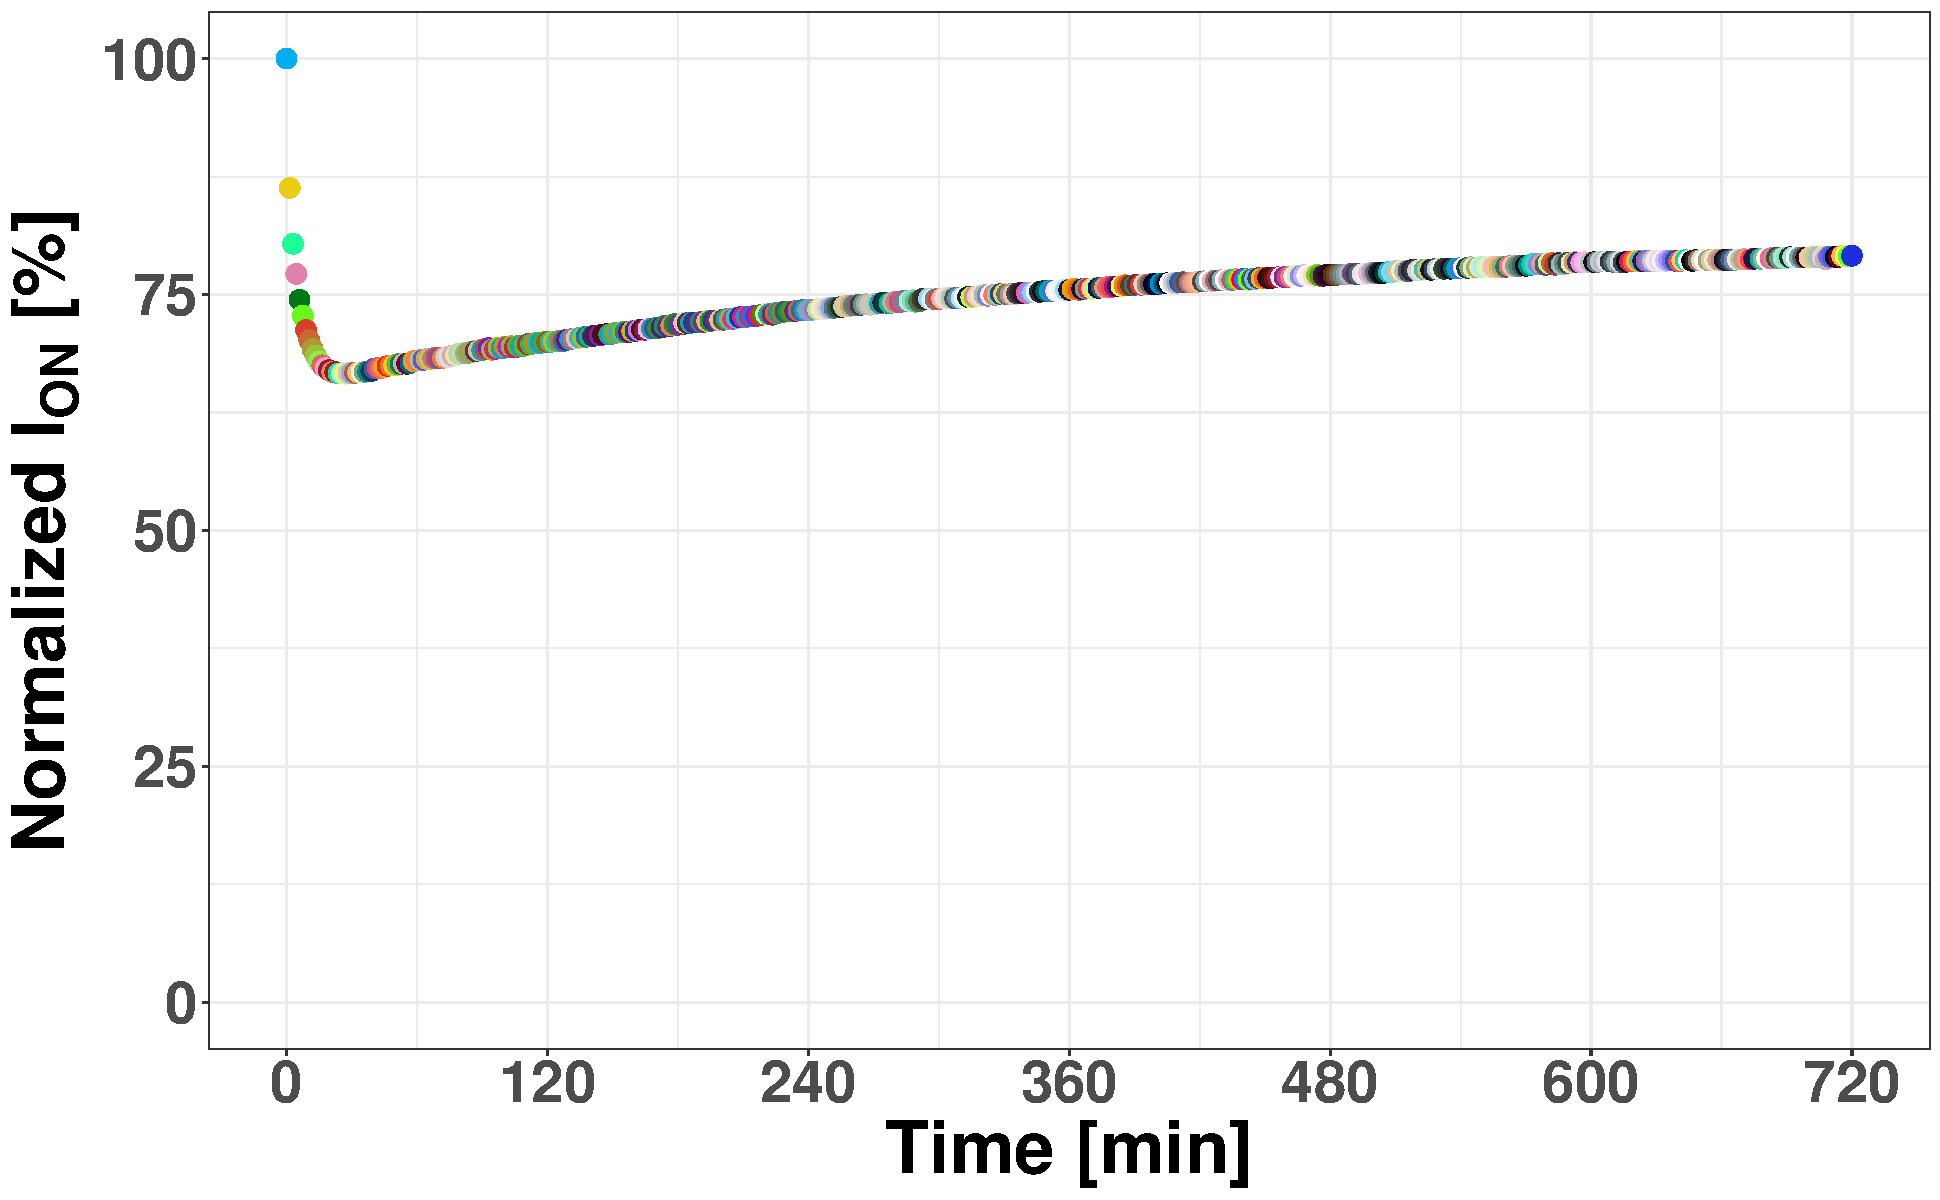
\includegraphics[width=0.45\textwidth]{figures/chapter3/EGFET/norm12h.pdf}%
        \label{fig:norm12h}
    }
    \caption{Normalized \ion{} for prolonged measurements. 
        (a) Experiments were carried out for \SI{4}{\hour} and the \ion{} was extracted; 
        (b) Similarly, more experiments were conducted over the span of \SI{12}{\hour}, extending beyond the standard experiment that takes place over \SI{60}{\min}. In both cases, the current continues to increase over time, demonstrating that the CNTs under the lipophilic membrane remain stable, even when exposed to extended environmental and electrical stress. This result confirms the long-term reliability of the devices, making them suitable for subsequent prolonged sensing applications.}
    \label{fig:normLong}
\end{figure}

The devices with the encapsulated channel demonstrate remarkable stability even over prolonged periods, as seen in Figure \ref{fig:normLong}. Indeed, measurements were carried out beyond the standard protocol, extending the collection of transfer characteristics for \SI{4}{\hour} (Figure \ref{fig:norm4h}) and later up to \SI{12}{\hour} (Figure \ref{fig:norm12h}). The \ion{} was extracted from the datasets and the trends analyzed: both plots reveal a continued increase in current over time, thus showing resilience well past the duration of a typical calibration curve in sensing applications. It is also important to observe that the current still follows a linear progression, even for these extended periods, thus ensuring the consistency required for EG-CNTFETs to be utilized effectively as sensor transducers.

\begin{figure}
    \centering
    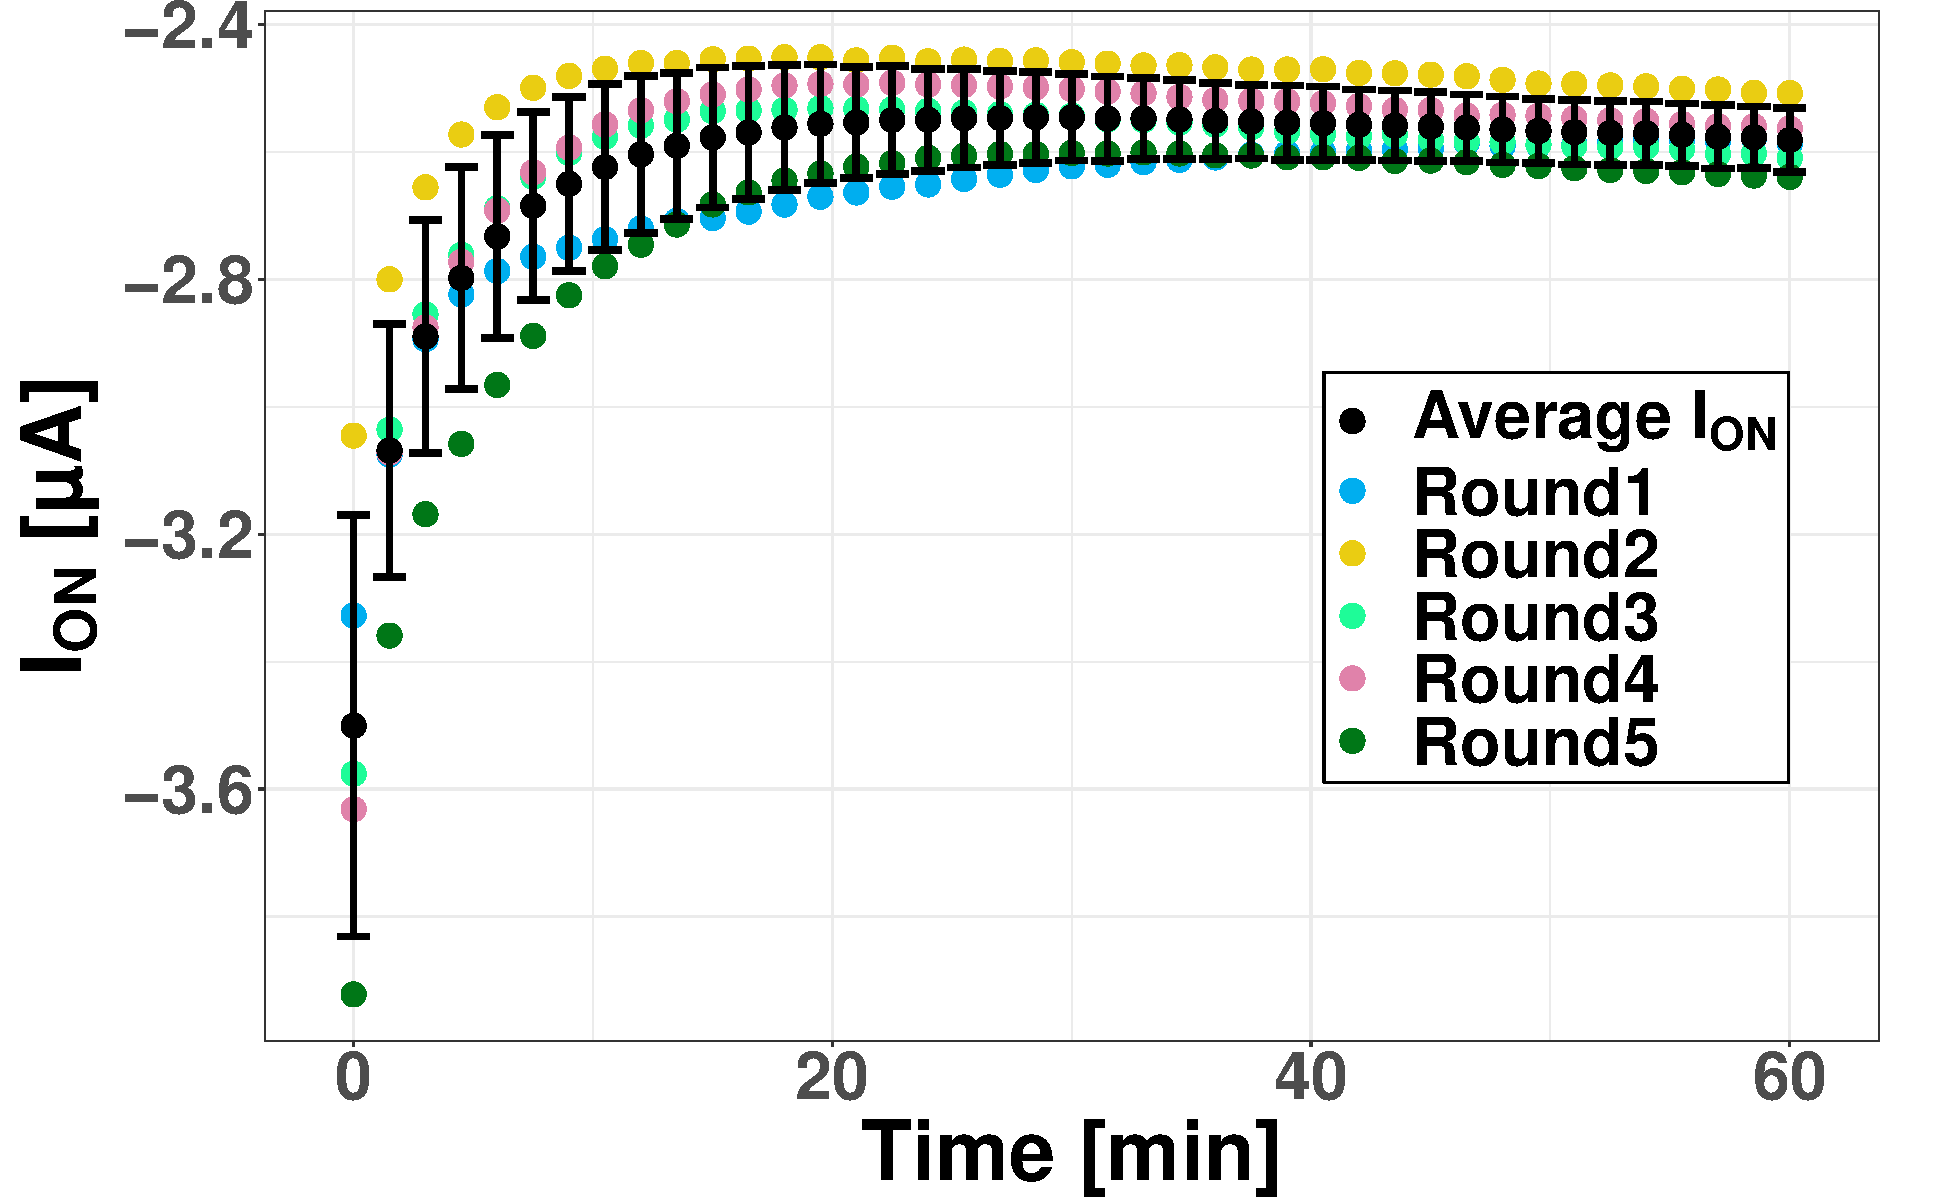
\includegraphics[width=0.45\textwidth]{figures/chapter3/EGFET/repMeas.pdf}
    \caption{\ion{} over multiple measurement cycles. The figure shows the \ion{} for a single device undergoing five consecutive transfer characteristic collections. The results demonstrate high reproducibility, with variability among the five cycles amounting to just \SI{2.67}{\%} after \SI{30}{\min} (the time necessary on average to reach an equilibrium), further reducing to \SI{1.93}{\%} after \SI{60}{\min}. This consistency highlights the reliability if the devices for repeated use in sensing applications.}
    \label{fig:repMeas}
\end{figure}

An additional test was conducted to test the resilience of the devices to multiple uses. To this end, the devices were subjected to five standard cycles of measurements (\SI{60}{\min}) and their performance was evaluated by extracting \ion{}. The results in Figure \ref{fig:repMeas} demonstrate that when the channel is covered by a lipophilic membrane, the EG-CNTFET devices maintain a stable and reproducible performance over multiple uses. Indeed, it is possible to see that while the standard deviation is very high at the beginning of the measurement, it decreases over time: after the \SI{30}{\min} required to reach the constant slope phase, the variability is \SI{2.67}{\%}, and it further improves after \SI{60}{\min}, being as low as \SI{1.93}{\%}. This is a promising outcome, as it indicates that the transducing component of the sensor can be reused without significant degradation. The ability to reuse the devices not only reduces costs but also electronic waste, making this approach more sustainable compared to single-use sensor platforms. These findings further support the feasibility of the encapsulation strategy for the development of EG-CNTFET-based sensors.

\begin{figure}
    \centering
    \subfloat[Average On/Off ratio]{
        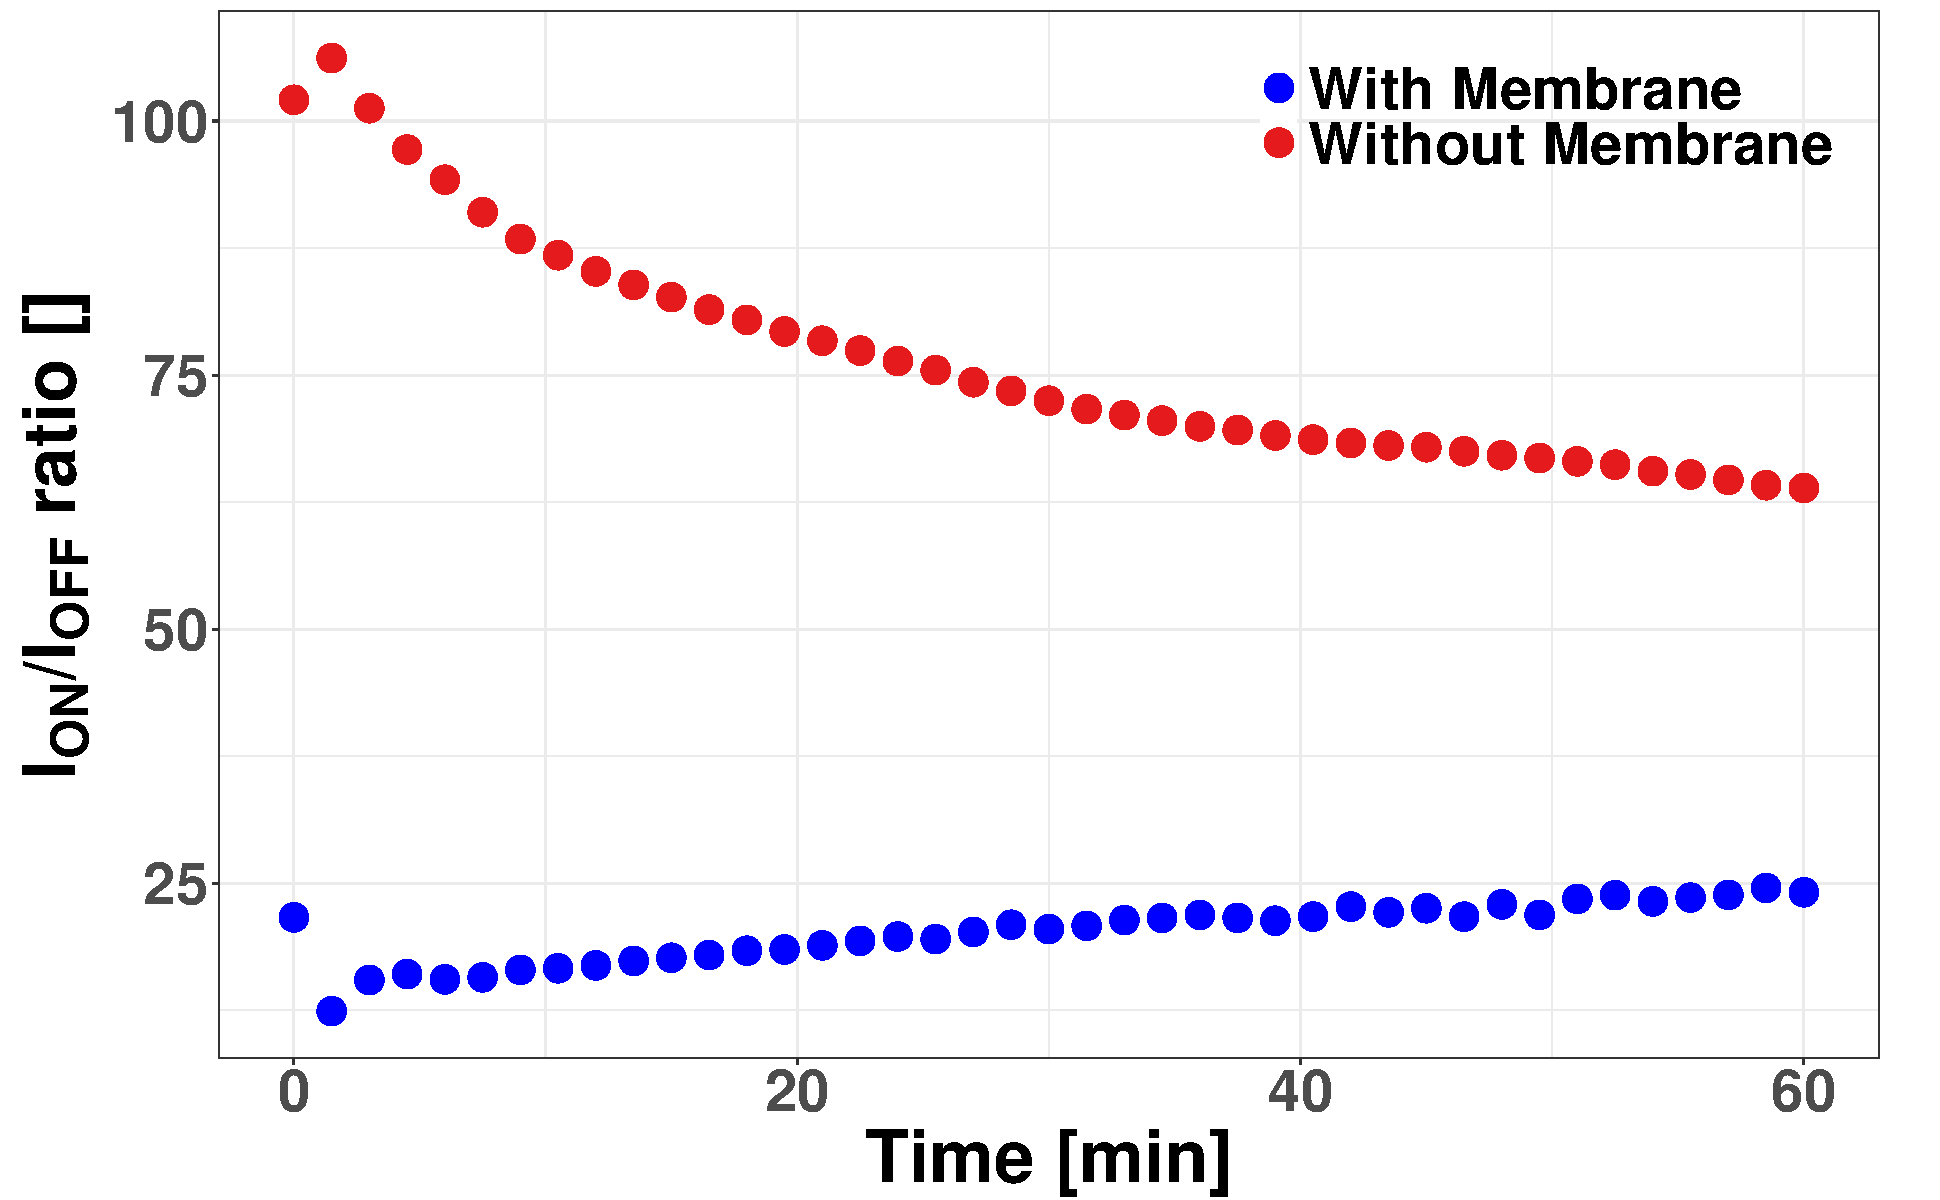
\includegraphics[width=0.45\textwidth]{figures/chapter3/EGFET/AvgOnOffRatio.pdf}
        \label{fig:avgOnOff}
    }
    \hfill
    \subfloat[Average threshold voltage]{
        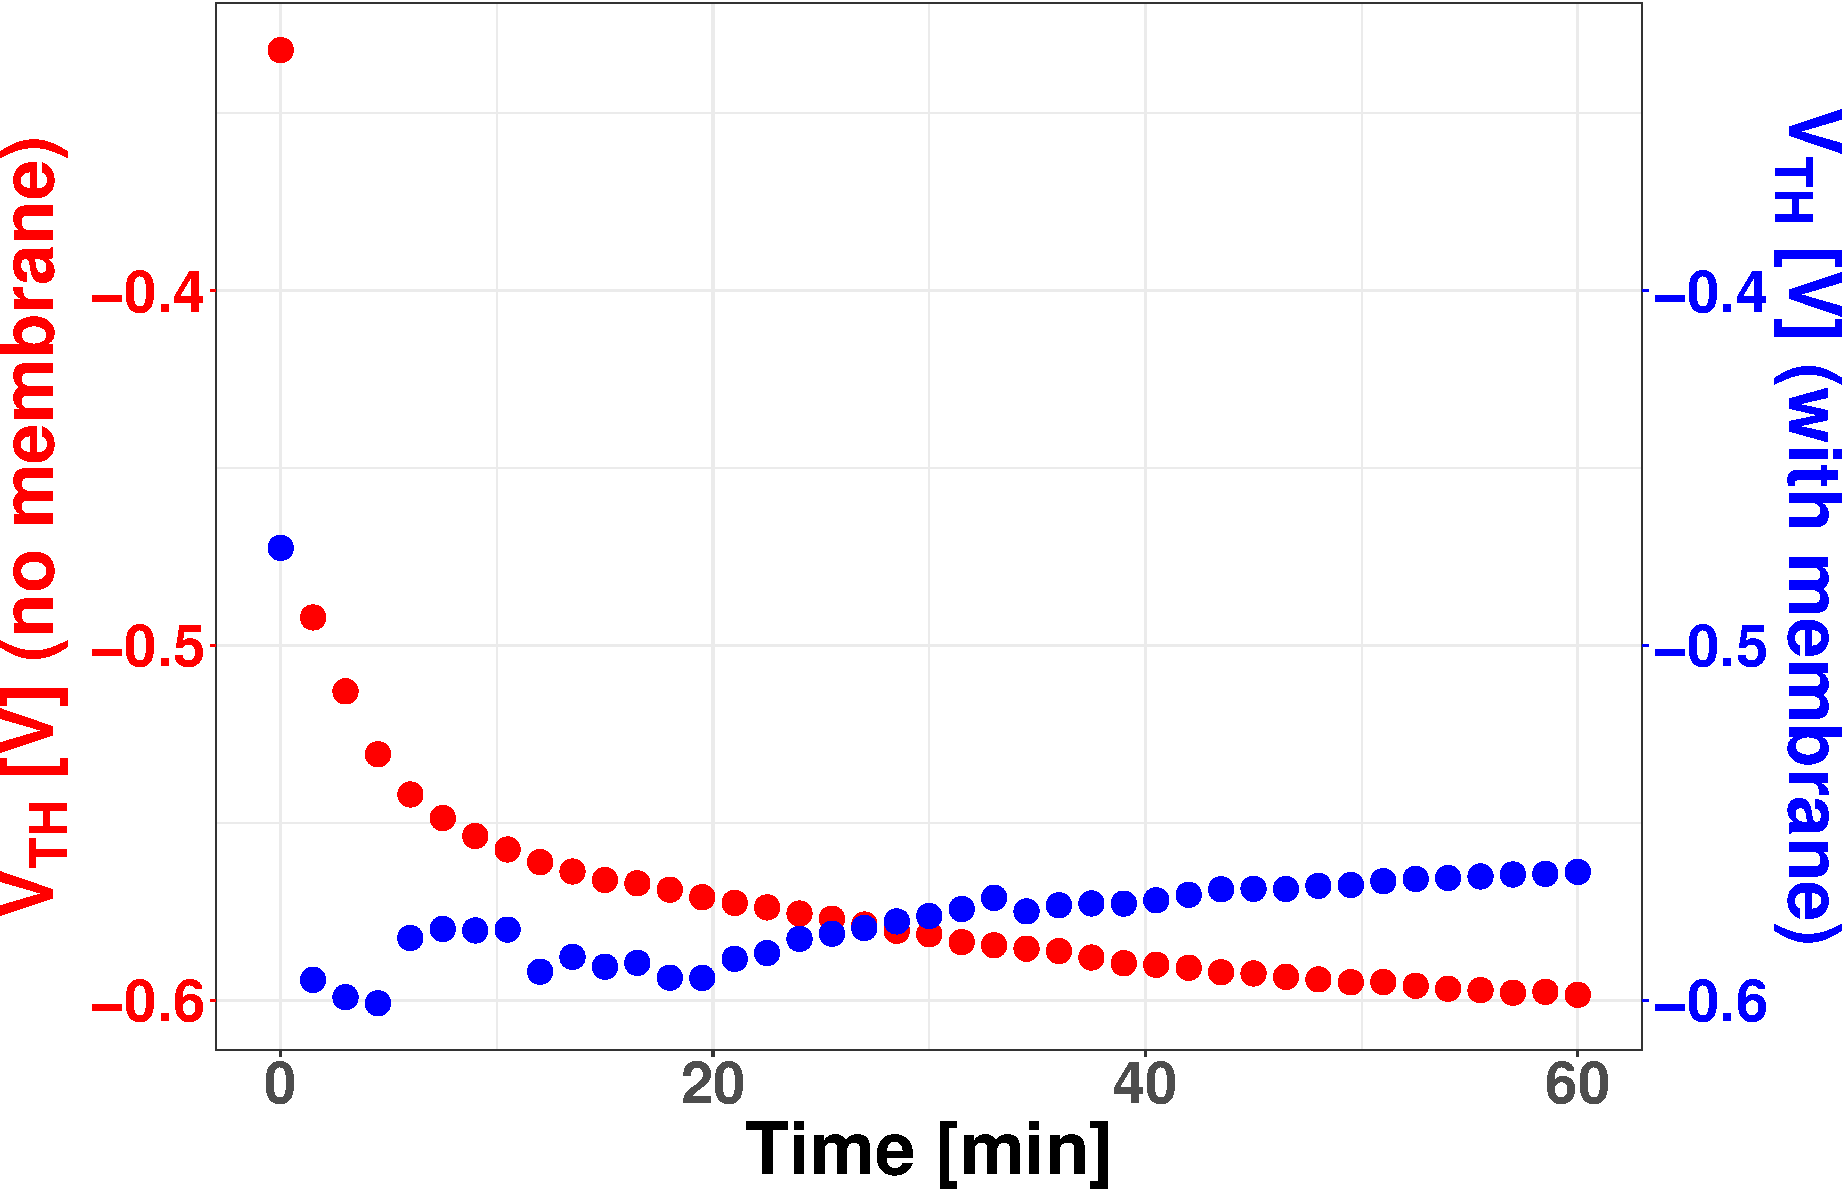
\includegraphics[width=0.45\textwidth]{figures/chapter3/EGFET/AvgVth.pdf}
        \label{fig:avgVth}
    }
    \caption{Comparison of the average of electrical parameters for device without the membrane ($N = 3$) and devices with the membrane ($N = 6$): (a) ON/OFF ratio and (b) threshold voltage.}
    \label{fig:avgParamsCfr}
\end{figure}

After this electrical characterization, parameters like the ON/OFF ratio (\ratio{}) and the threshold voltage (\vth{}) were calculated, to gather additional knowledge of device performance. In particular, Figure \ref{fig:avgOnOff} compares the trends of the ON/OFF ratio for devices without and with the lipophilic membrane. The bare devices exhibit a significant decrease in the ON/OFF ratio, dropping from 100 to 60. This reduction indicates a worsening in device performance over time. In contrast, devices with the encapsulated channel display a markedly different trend. After an initial drop from 17.63 to 9, the ON/OFF ratio exhibits a continuous linear increase, eventually reaching 24.51. This improvement suggests that the encapsulated devices have an enhanced performance at the end of the measurements.
Figure \ref{fig:avgVth} displays the average \vth{} for both bare (red) and encapsulated (blue) devices, showing a comparison of the trends. It is immediately clear that this parameter is more easily comparable for the two devices than the ON/OFF ratio, as it has the same order of magnitude. The trends that the parameters display, though differ for the two cases: for the unprotected devices, \vth{} continuously increases in modulus, meaning that the device requires a higher gate voltage to reach the conductive state; indeed, the \vth{} at the beginning amounts to \SI{-0.421}{} $\pm$ \SI{0.105}{\V} and at the end it is \SI{-0.613}{} $\pm$ \SI{0.0225}{\V}. Conversely, the \vth{} of membrane-protected devices
follows a similar trend to the \ion{}, in that it starts high, then drops very quickly at the beginning, only to linearly start increasing again. In this case, the \vth{} starts at \SI{-0.487}{} $\pm$ \SI{0.109}{\V} and ends at \SI{-0.570}{} $\pm$ \SI{0.0201}{\V}. Maintaining a lower \vth{} is particularly relevant for sensor applications, ensuring improved reproducibility, and lower power consumption over extended use. These findings further highlight the benefits of incorporating a protective membrane to enhance the stability and longevity of EG-CNTFETs.
